% ---------------------------------------------------------------------------
% Compact narrative draft of the main text (Sections 1-6).
% Companion: theory_appendix_main_results.tex holds every statement in full,
% in derivation order.  Here propositions are stated only where they carry the
% story; everything else is a pointer.
%
% Figure plan (3 figures):
%   Fig 1  neuronal results (top row) + linear recapitulation (bottom row)
%   Fig 2  pixel ridge: landscape + CV path
%   Fig 3  feature ridge: dependency graph + null rotation + biological validation
%   wrapfig  iso-error geometry + ridge path (Sec 3)
% ---------------------------------------------------------------------------

\begin{abstract}
Deep neural networks are increasingly used both as encoding models of visual cortex and as controllers that synthesize images to drive neural responses toward desired states. Recent \textit{in vivo} experiments reveal a striking dissociation: models with nearly identical held-out accuracy can generate qualitatively different stimuli and differ sharply in control, and these differences track input-gradient structure better than predictive accuracy. We develop a geometric and analytical account of this phenomenon in a linear teacher–student model. The key is that control creates a self-generated distribution shift. Natural-image generalization, self-accentuation, and peer review evaluate the same fitted predictor under three different input distributions; correspondingly, their equal-error sets in weight space are ellipsoids, spheres, and hyperplanes.
% Generalization weights estimation error by the data covariance, whereas self-accentuation exposes it along the model’s own fitted direction in Euclidean geometry.
Using deterministic equivalents for ridge regression, we show that prediction-optimal and control-optimal regularization satisfy different spectral conditions, so cross-validation can leave large control error when responses are noisy and inputs are anisotropic. Extending the analysis to fixed linear feature maps, we construct a prediction-preserving gauge family with identical generalization and cross-validated regularization but arbitrarily different control. Control is most fragile when feature directions that survive regularization backpropagate into low-variance, high-spatial-frequency image directions. The resulting gradient-geometry factor extends to nonlinear networks as a Jacobian-based diagnostic and predicts across-model variation in \textit{in vivo} control better than held-out prediction error. Thus predictive accuracy alone cannot certify control; the model’s gradient geometry or generated stimuli must also be evaluated.
% Deep neural networks are increasingly used both as encoding models of visual cortex and as controllers that synthesize images to drive neural responses toward desired states. Recent \textit{in vivo} experiments show that, models with similar held-out accuracy in predicting visual-neuron responses can differ sharply in the features they rely on and in their ability to generate stimuli to control those neurons. Moreover, the control success is more associated by the structure of a model's input gradient than its predictive accuracy.
% We develop a geometric and analytical account of this prediction--control dissociation using a linear teacher--student model.
% Classic generalization evaluates a fitted predictor on the natural-image distribution; model-based control evaluates it on a path along its own fitted direction. Such difference in evaluation distribution leads to different iso-error geometry in the weight space.
% %feature accentuation evaluates it on a distribution generated along its own fitted direction.
% % This change of distribution gives control error, $R^2$, and response slope a different dependence on estimation error than test loss: prediction weights error by the data covariance, control counts it in Euclidean geometry.
% Using deterministic equivalents for ridge regression we show that prediction-optimal and control-optimal regularization obey different spectral conditions, so cross-validation can leave large control error under noisy, anisotropic data. Extending the analysis to fixed linear feature maps, prediction depends only on the feature covariance and its alignment with the teacher, whereas control additionally depends on the map's input-gradient geometry. We construct a gauge family of feature maps with identical generalization performance, but arbitrarily different control. Control is most fragile when the feature directions that survive regularization backpropagate into low-variance, high-spatial-frequency image directions. The resulting gradient-geometry factor extends to nonlinear networks as a diagnostic and predicts the variation of \textit{in vivo} control capability of models better than held-out prediction accuracy.
\end{abstract}

% suggested new abstract content - maybe something in here is useful
% Deep neural networks are increasingly treated as models of primate visual processing and used to predict neural responses in visual cortex. These mappings from image space to brain activity, known as encoding models, can also be used to attempt neural control, by synthesizing images that are predicted to drive neural firing into a chosen state. Surprisingly, recent large-scale in vivo experiments found that many leading models with nearly identical held-out predictive accuracy over natural images differ substantially in their capacity for neural control. Here we develop a geometric and analytical account of this prediction-control dissociation. Using a linear model of a neuron whose true preferences are known, we make two key observations. First, prediction and control evaluate the same model on different inputs. Natural image prediction relies on images that vary widely along some dimensions and hardly at all along others, with errors along rarely explored directions not reflected in generalization scores.  Controller stimuli instead exaggerate the hypothesized directions of neural sensitivity, directly targeting the underexplored directions and exposing exactly those errors. Second, the ridge regularization best for prediction generally differs from the one best for control, so standard cross-validation can leave large control errors, especially when data are noisy. Extending the theory to models built on fixed features, we show that equally predictive models can differ arbitrarily in control, depending on how much their input gradients rely on these neglected directions. Measuring this reliance yields a diagnostic that can be computed before any control experiment. On the neural dataset that motivated this study, this diagnostic predicts which models will best control each neural site, while natural image predictivity carries almost no information. These results imply that models selected for natural-image predictivity, as in most current benchmarks, may not support effective control, and that future evaluations should test a model's gradients or generated stimuli directly.


\section{Introduction}
A good predictive model of a neuron can, in principle, be used as a \textit{model-based} controller: if $f(\x)$ predicts the response of a neuron to an image $\x$, one can synthesize images that drive $f$ to a target level and present them to the subject to modulate neuronal state.
Aside from model-free generative search \citep{ponce2019evolvingImages,xiao2020xdream}, model-based control of visual neurons has been successfully pursued across species \citep{bashivan2019neuralPopulationControl,walker2019inceptionLoops}. Recently, \citetPW scaled this paradigm into a benchmark of many deep-network encoding models and uncovered three puzzles: Encoding models that are nearly indistinguishable on predicting held-out natural images generate visibly different stimuli and differ several-fold in how well those stimuli modulate the neuron \textit{in vivo}; models that fail to control can still recognize the successful stimuli of other models; and the best predictor of control success is not accuracy but the spectral structure of the model's input gradient.

% We argue that none of this requires nonlinearity, depth or biology.
We argue that these phenomena arise already in linear models, from a single fact: \emph{control evaluates a model on a distribution the model generates itself}. Held-out prediction measures weight error in the metric of the data covariance $\Sigma$, which suppresses low-variance directions; accentuation moves along the fitted weight itself and therefore measures the same error in Euclidean geometry, where nothing is suppressed. For natural images, whose covariance spectrum decays over many orders of magnitude, this is the difference between not seeing an error and being dominated by it.

Our contributions are:
\textbf{(I)} a formulation of generalization, self-accentuation and peer review as evaluations of one predictor under three input distributions, with their equal-error sets (ellipsoid, sphere, hyperplane) exposing the dissociation geometrically (Sec.~\ref{sec:setup});
\textbf{(ii)} deterministic equivalents for pixel-space ridge regression showing that prediction-optimal and control-optimal penalties satisfy different spectral conditions, so cross-validation in anisotropic data and teacher leaves a computable residual control error (Sec.~\ref{sec:pixel});
\textbf{(iii)} for ridge regression on a fixed linear feature map, a separation of the summary statistics that determine prediction from those that determine control, and a gauge family of feature maps with identical generalization but arbitrarily different control (Sec.~\ref{sec:feature});
\textbf{(iv)} a response-independent gradient-geometry factor $T_F$ that identifies fragile feature maps, extends to nonlinear networks as a diagnostic, and recovers model ordering in the neuronal control data.
All statements are proved in the appendix, where we also restates every result in derivation order (App.~\ref{sec:app-main-results}); numerical validation against Monte Carlo accompanies each section. %and natural-image regression

% \paragraph{Related work.}
% High-dimensional ridge regression under anisotropic covariance is classical \citep{dobriban2018high,hastie2022surprises}, and deterministic equivalents for its risk are standard \citep{bai2010spectral,couillet2011random}; we use this toolkit but change the evaluation distribution from the training law to a model-generated path. Optimizing inputs against a fitted model is the setting of feature visualization and accentuation \citep{olah2017feature,hamblin2024feature}, adversarial examples and performative prediction; our contribution is a solvable model in which the resulting distribution shift is computed rather than assumed. %Model-based closed-loop neuroscience \citepPW\ supplies the phenomena.
\paragraph{Related work.}
Encoding models built on deep networks now predict cortical responses so similarly that benchmarks no longer rank them \citep{yamins2014performanceOptimized,guclu2015deepGradientComplexity,cadena2019deepConvolutionalV1,schrimpf2018brainscore,conwell2024inductiveBiases}. Read one way this is convergence \citep{huh2024platonicRepresentationHypothesis,kapoor2026convergentLearning}; read another it is a weak test, answered by constraining the mapping \citep{prince2024sparsePositiveAlignment} or by seeking stimuli that split models apart \citep{golan2020controversialStimuli,feather2023modelMetamers,rajalingham2018large,geirhos2019imagenetTextureBias}. Closed-loop control is one limit of that strategy: the model writes the stimulus and the neuron grades it \citep{ponce2019evolvingImages,xiao2020xdream,bashivan2019neuralPopulationControl,walker2019inceptionLoops,prince2026parametric}. Optimizing an input against a fitted model likewise underlies feature visualization \citep{olah2017feature,hamblin2024feature,fel2023magnitudeConstrainedOptimization} and adversarial attack \citep{nguyen2015deepNeuralFooled,goodfellow2015explainingAdversarial,madry2018towardsResistant}, where robustness has been tied to alignment \citep{guo2022adversariallyTrainedNeuralRepresentations,dapello2020simulatingV1,taori2020measuring}.
In each case the test distribution is created by the model under test, which we make analytical.
Classic theory characterizes ridge risk under anisotropic covariance and signal--spectrum alignment \citep{dobriban2018high,hastie2022surprises,mei2022generalization,mel2021highDimensionalRegression}, as well as generalization and optimal regularization under an externally specified train--test distribution shift \citep{canatar2021outOfDistribution,tripuraneni2021covariateShift,patil2024optimalOODRidge}. We instead study a self-generated shift: the test distribution is supported on an optimization path created by the fitted predictor itself.
%  carrying theory of ridge risk under anisotropic covariance \citep{dobriban2018high,hastie2022surprises,mei2022generalization,bai2010spectral,couillet2011random} off the training law  and onto the model's own path.

\section{Prediction and control dissociate in neurons and in linear regression}
\label{sec:phenomena}

\begin{figure}[t]
    \centering
    \vspace{-14pt}
    % 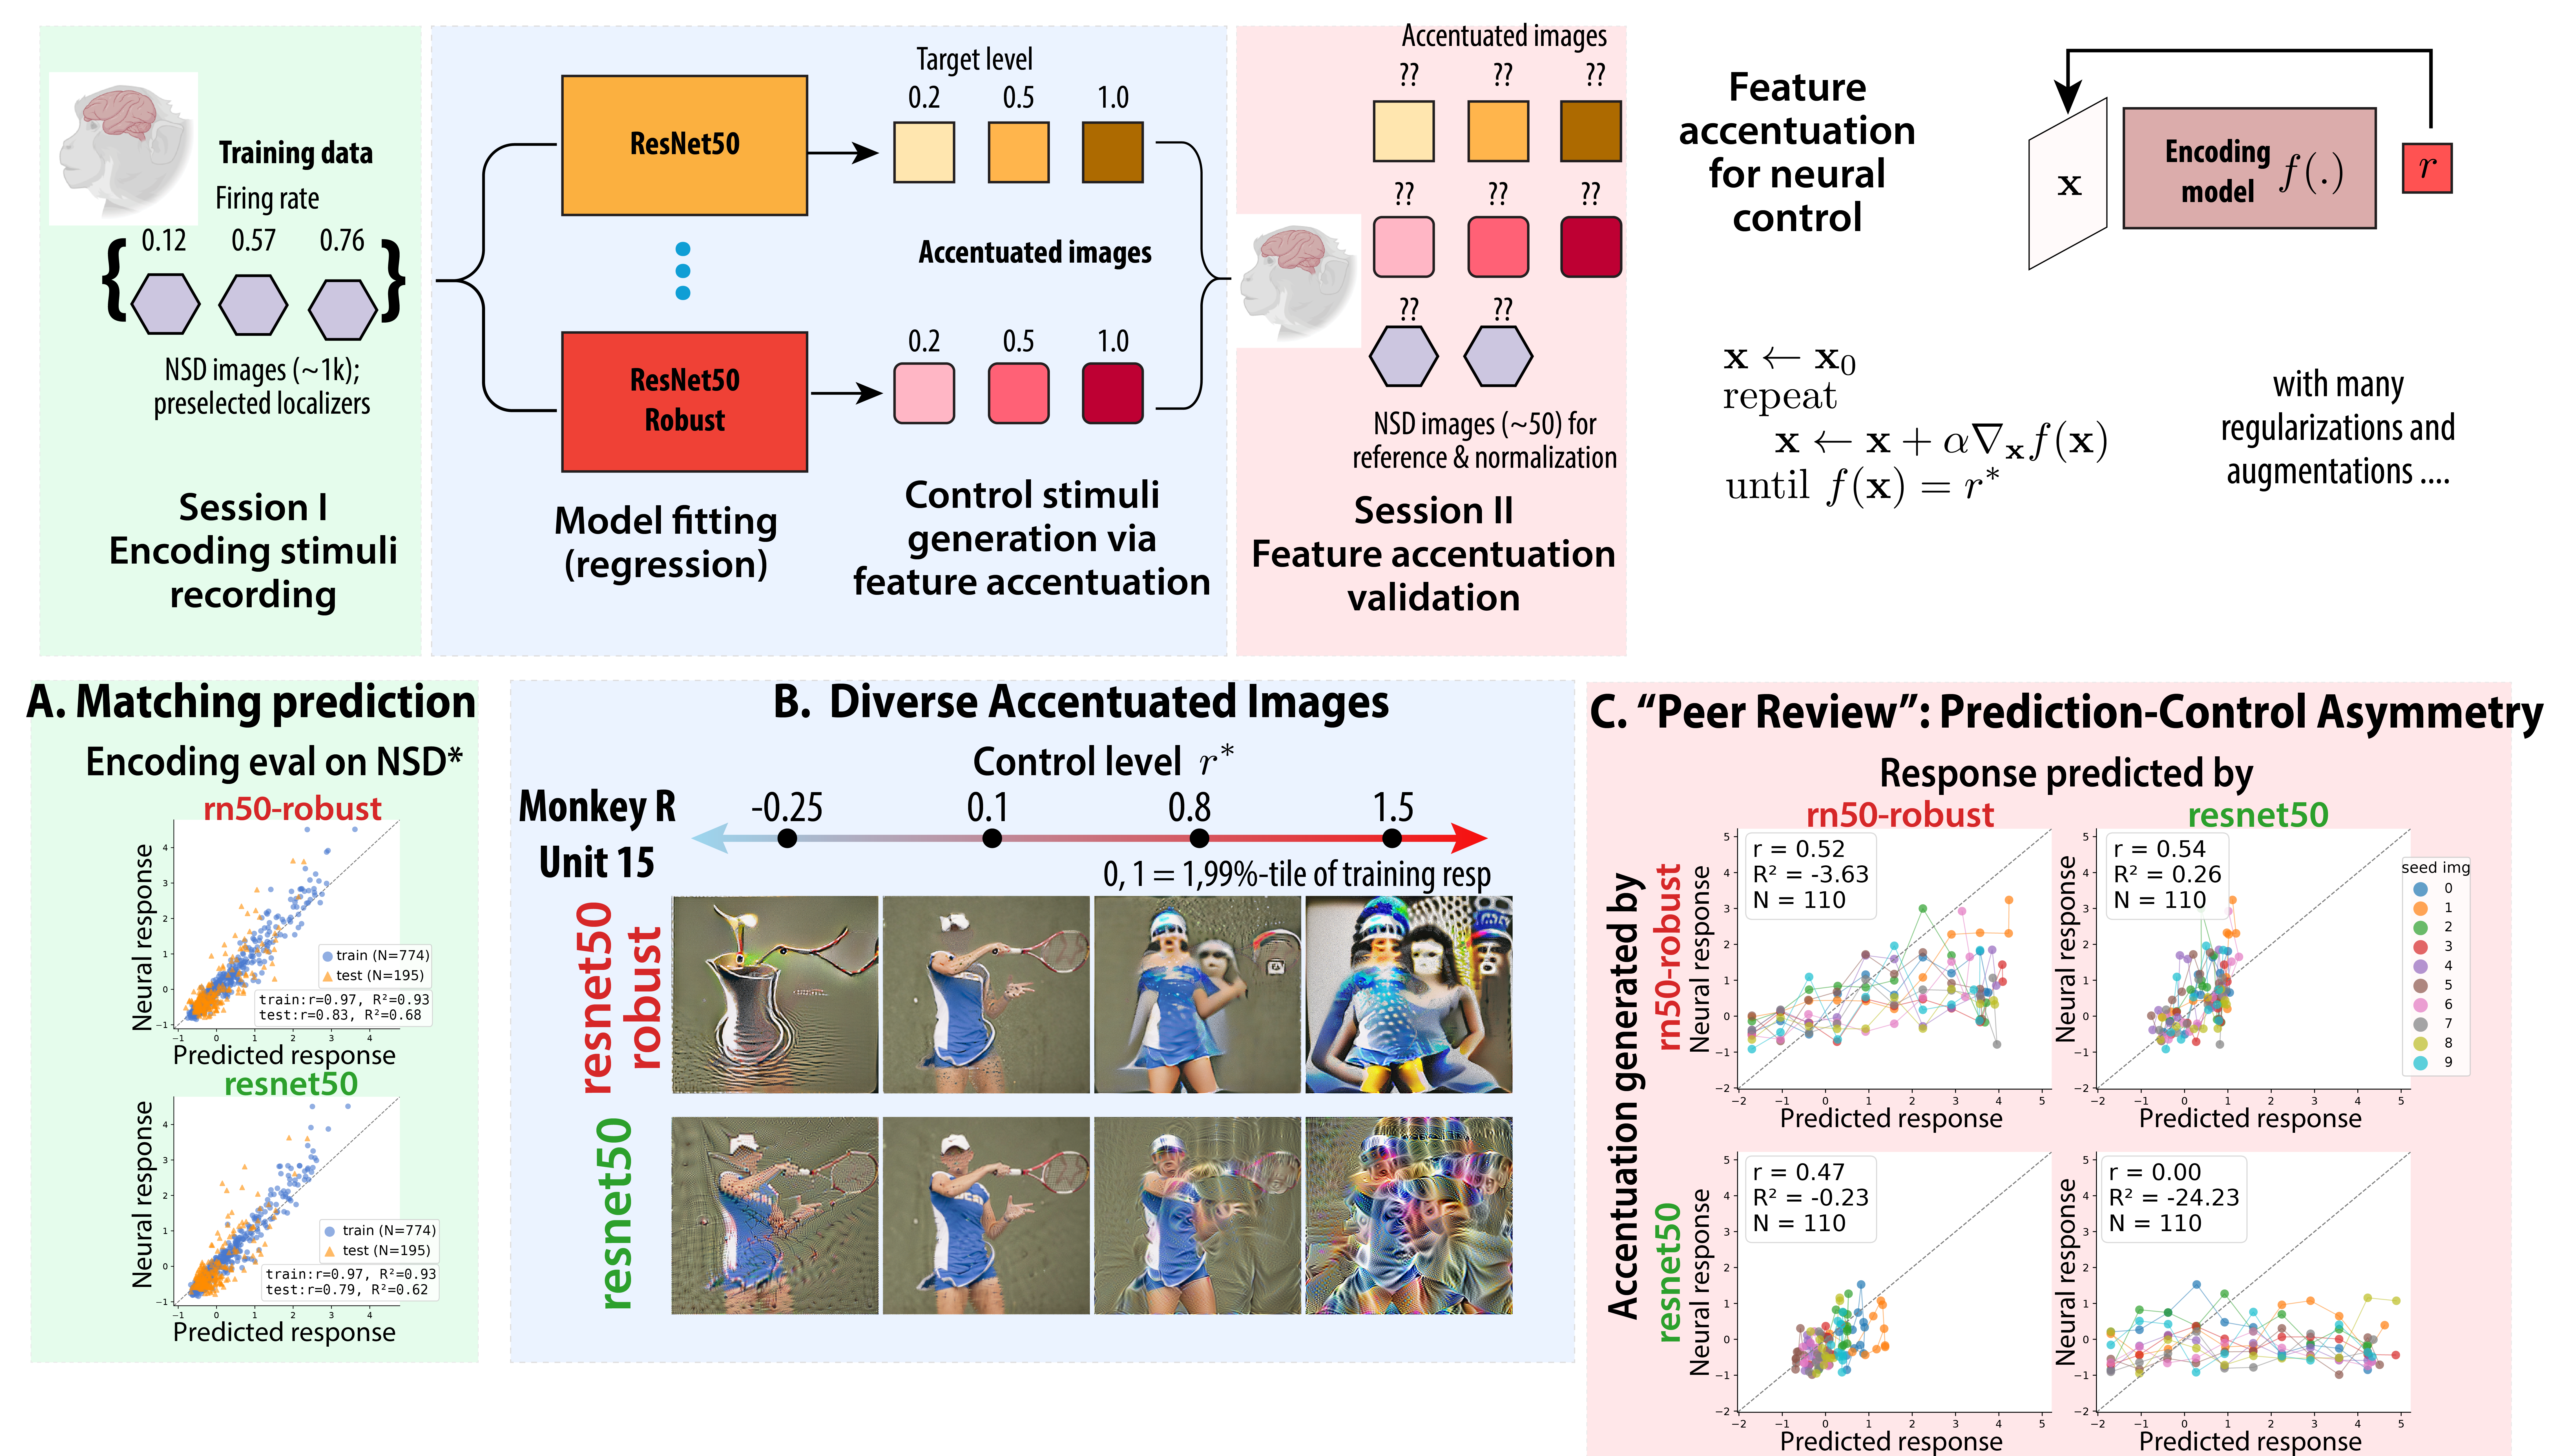
\includegraphics[width=\linewidth]{figures/Figure_NeuroCtrl_results.png}\\[2pt]
    % \vspace{-5pt}
    % 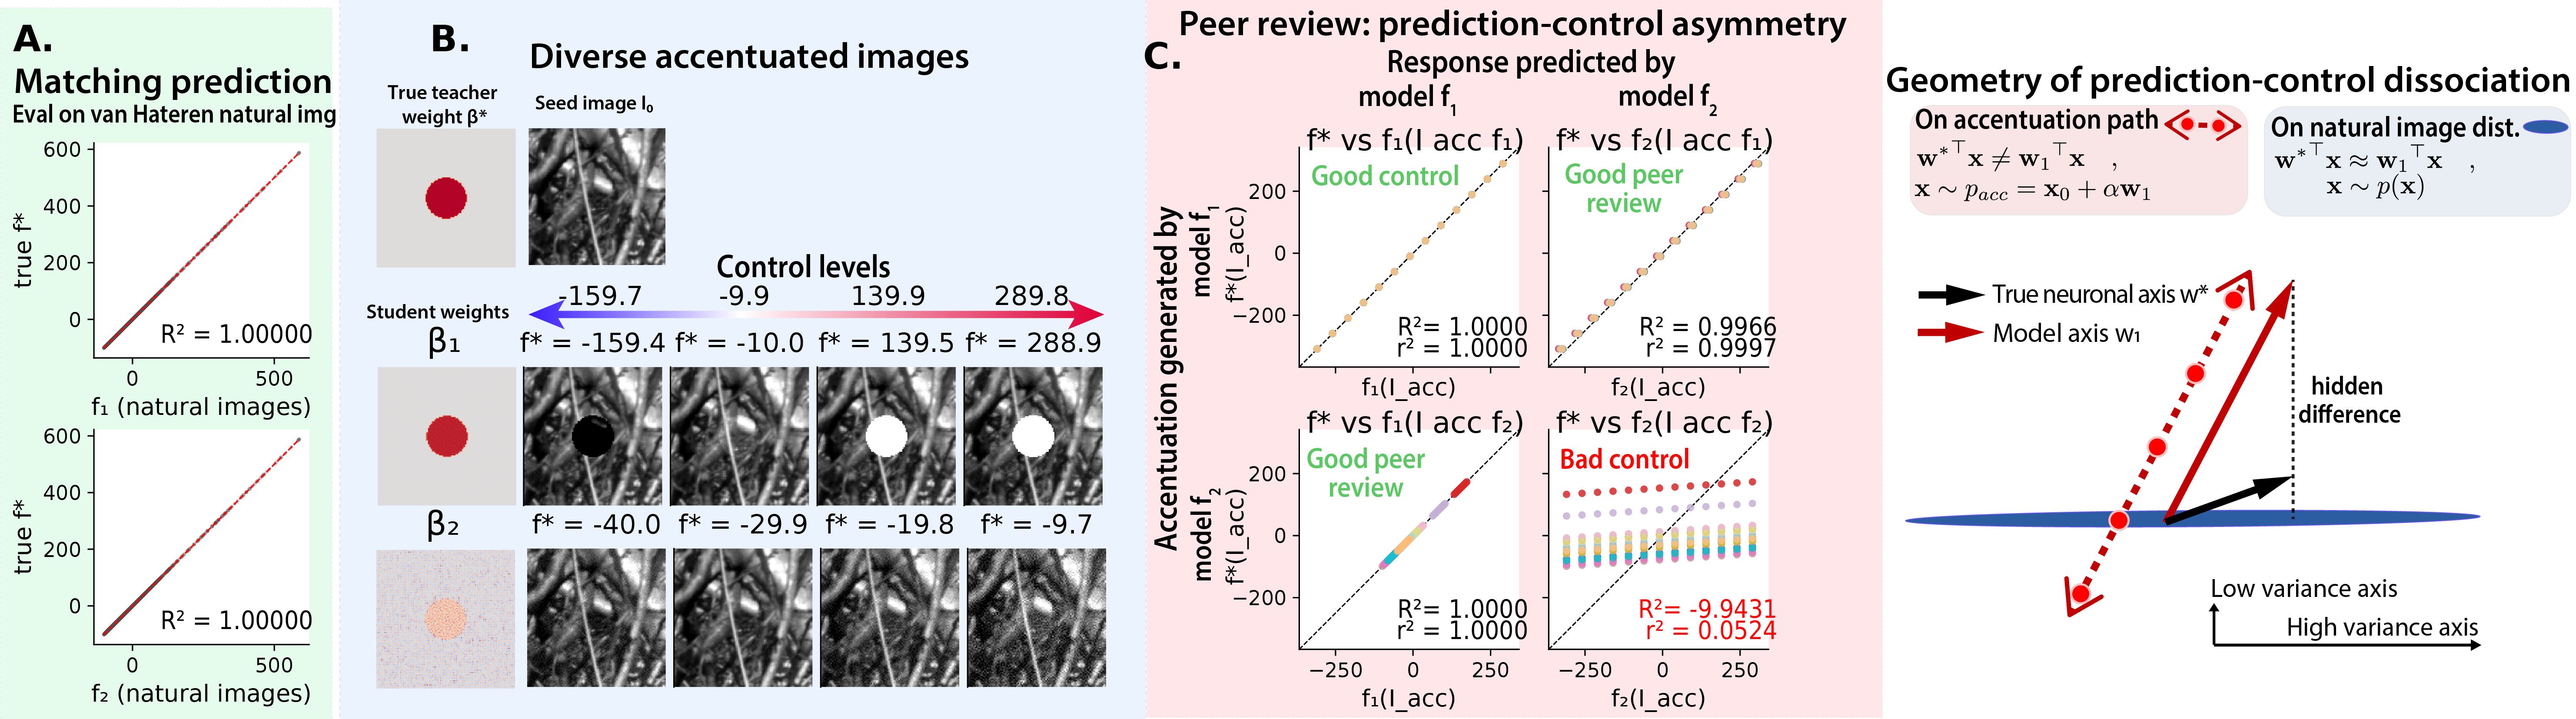
\includegraphics[width=\linewidth]{figures/Figure_LinearToyModel-04.png}
    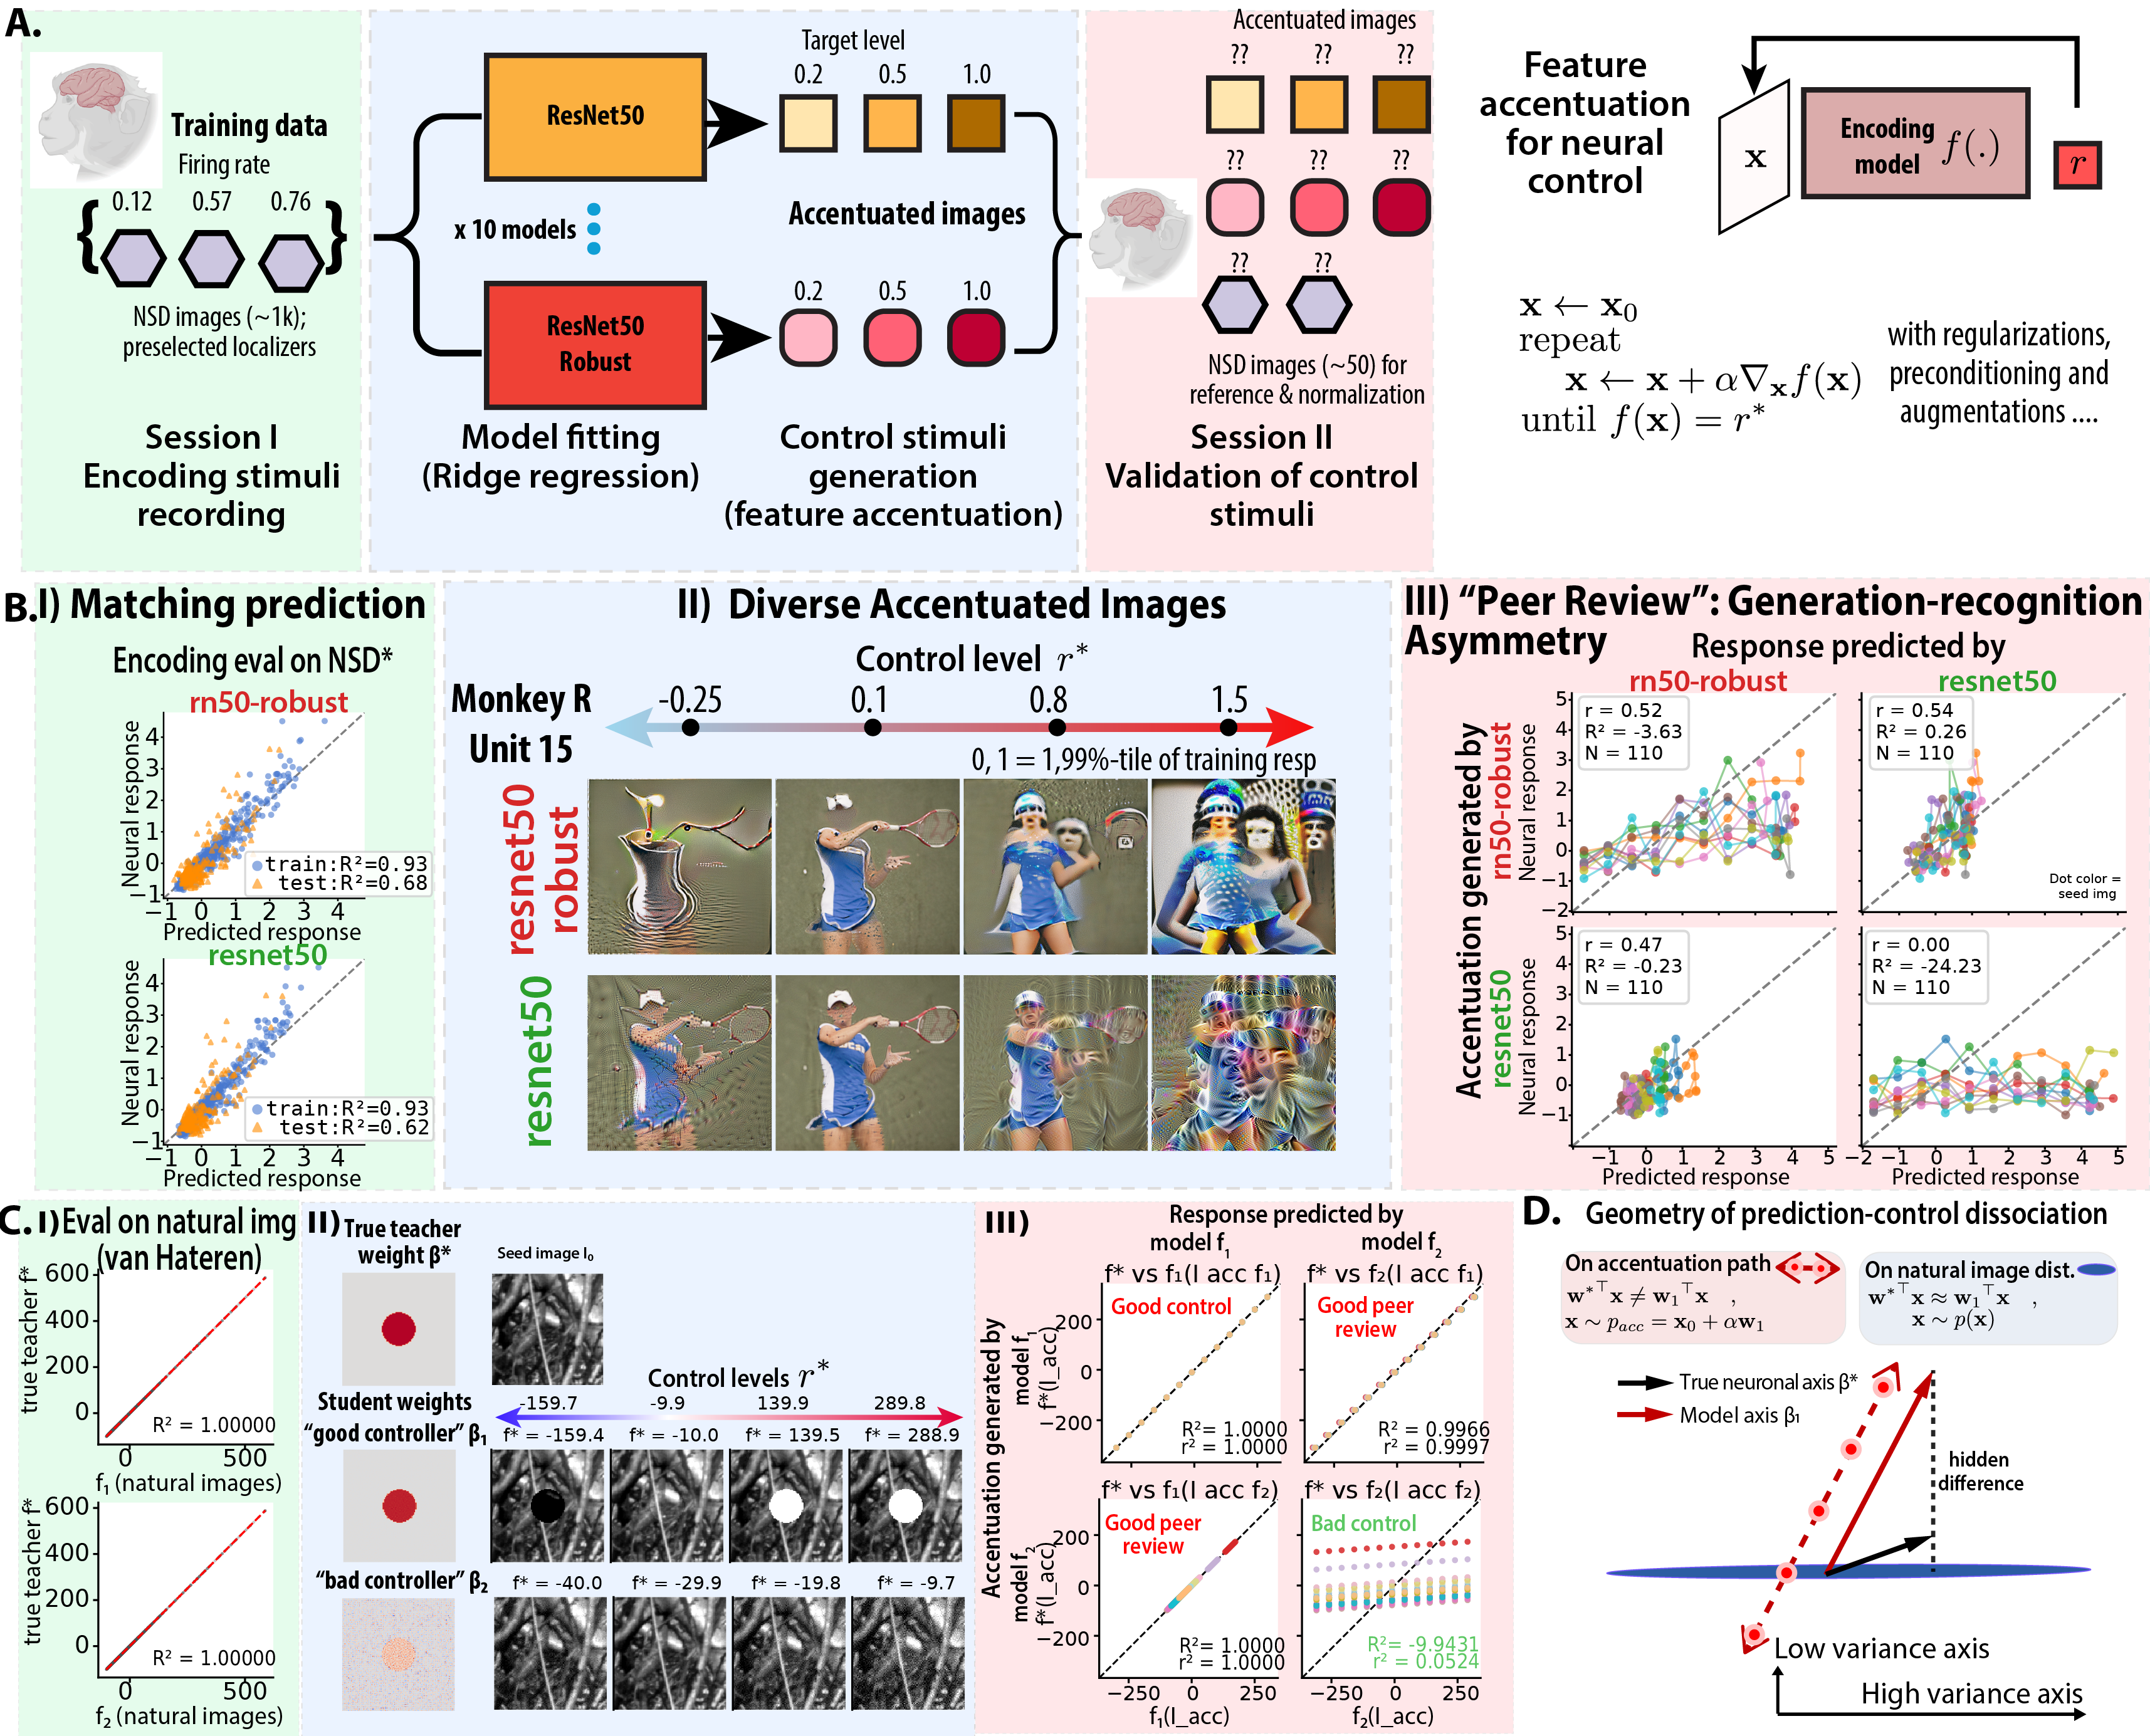
\includegraphics[width=\linewidth]{figures/Figure_NeuroCtrl_results_Neuro-linear-compose.png}
    \vspace{-10pt}
    \caption{\textbf{The dissociation of prediction and control in neurons and in a linear teacher--student model.}
    \textbf{A.} Closed-loop experiment of \citetPW. Encoding models are fit to responses to natural images, generate accentuated images for graded target responses, and are tested in a second session.
    \textbf{B.}
    \textbf{I}~Two models predict held-out natural-image responses equally well.
    \textbf{II}~Their accentuations from the same seed differ visibly.
    \textbf{III}~When each model evaluated on the other's images (\textit{peer review}), the weak controller (RN50) tracks neuronal responses on the strong controller's (RN50-robust) images but its own images barely modulate the neuron. % Only RN50-robust modulates the neuron.
    \textbf{C.}: two linear students of a linear teacher (a disk-shaped weight on van~Hateren images), weight differing along low-variance image directions, reproduce I-III qualitatively.
    \textbf{D.}: prediction on natural data hides weight error in small variance dim; the accentuation path exposes the hidden Euclidean difference.
    Methods see App.~\ref{sec:app-methods-neural-data}, ~\ref{sec:app-methods-toy} }
    %Details: App.~\ref{sec:app-methods-neural-data} (neurons), App.~\ref{sec:app-methods-toy} (linear model).}
    \label{fig:phenomena}
\end{figure}


\citetPW   used the following closed-loop paradigm (Fig.~\ref{fig:phenomena}, top): responses of visual cortical sites (V3/V4--IT, 25 sites in 5 macaques) to $\sim$1000 naturalistic images were recorded; for each site, ten encoding models were fit by ridge regression on the top 750 PCs of features from ten deep network backbones, with penalty and per-site layer chosen by cross-validation; using \emph{feature accentuation} \citep{hamblin2024feature}, each model optimized an image using a variant of gradient ascent, and then synthesized images that drive its own prediction to eleven target levels from ten seed images (Fig.~\ref{fig:phenomena}\textbf{A}); and the images were presented to the same sites in the \textit{control session}. The control is successful if the proposed images evoked neural activations as predicted (data and models: Apps.~\ref{sec:app-methods-neural-data},~\ref{sec:app-methods-models}). Three observations motivate this paper.

\paragraph{Similar prediction, divergent control.}
The trained models were tightly matched on held-out natural images (Fig.~\ref{fig:phenomena}\textbf{B.I}), yet the slope and correlation between predicted and measured responses to their own accentuated images varied widely across models, with far larger spread than on natural images. Many models reached their target \emph{predicted} response by adding texture and high-spatial-frequency structure that left the neuron largely unmoved (Fig.~\ref{fig:phenomena}\textbf{B.II}).

\paragraph{Recognition without generation.}
Presenting model A's images to model B (``peer review'', Fig.~\ref{fig:phenomena}\textbf{B.III}) shows an asymmetry: a model whose own images fail to modulate the neuron still predicts the neuronal responses to a successful model's images with good correlation and better $R^2$ than the generator itself. Models can recognize good control stimuli that they cannot produce.

\paragraph{Control tracks input-gradient structure.}
Across the 250 site--model pairs, control success is predicted by the spectral profile of the model's input gradient $\nabla_\x f$: models whose gradients concentrate power at low spatial frequencies, like natural images, control better. The two adversarially trained models are the strongest controllers, but the association persists without them \citepPW.

These phenomena are puzzling at first glance, but linear models on natural images reproduce all three observations (Fig.~\ref{fig:phenomena}\textbf{C}). We construct the bad controller to deviate from the teacher along the lowest-variance, high-spatial-frequency directions of the image covariance, the good controller to deviate mildly along mid-band PCs; then matched prediction, diverse accentuations, unequal control and good peer review all follow. Dissecting this idealistic set up, the rest of the paper explains why \textit{finite-sample} regression on \textit{noisy responses} produces such errors, why \textit{cross-validation does not remove them}, and how \textit{feature maps} can amplify the dissociation.

% These phenomena are puzzling at first glance, though we show, linear models on natural images can reproduce all three observations (\red{
% bottom, Fig.~\ref{fig:phenomena}}).
% We constructed the bad controller to have weight error along low-variance directions of the image covariance (high spatial frequency), while the good controller has weight error more along the high eigenspace. Then matched prediction on natural data; diverse generated images; unequal control outcomes and relatively good peer reviews all emerge from it.
% This shows the same symptom can emerge without deep network, nonlinearity or neurons.
% Dissecting this idealistic set up, the remainder of the paper explains why \textit{finite-sample} regression on \textit{noisy responses} produces this failure, why \textit{cross-validation does not eliminate it}, and how \textit{feature maps} introduce additional degrees of freedom that can greatly amplify the prediction--control dissociation.


\vspace{-15pt}
\section{Three evaluations, three geometries of one predictor}
\label{sec:setup}

\paragraph{Teacher and student.}
We idealize a visual neuron as a noisy linear teacher, its encoding model as a linear student, and natural image inputs as $\x\in\R^d,\x\sim\mathcal N(0,\Sigma)$, a centered Gaussian distribution with structured covariance $\Sigma=\sum_ks_k\uvec_k\uvec_k^\top$.
A linear teacher with weight $\bstar=\sum_kb_k\uvec_k$ produces noisy responses $y=\x^\top\bstar+\sigma\epsilon$, $\epsilon\sim\mathcal{N}(0,1)$, and $S:={\bstar}^\top\Sigma\bstar$ is the noiseless natural response variance.
The student is $f(\x)=\x^\top\bhat$, fitted from $n$ pairs $(X,\mathbf y)$; for linear feature-space students (Sec.~\ref{sec:feature}) $\bhat$ is the effective pixel weight $F^\top\hat w$, which is also the gradient $\nabla_\x f$.

\paragraph{Three distributions.}
Generalization evaluates $f$ on fresh natural inputs, $\x\sim\mathcal N(0,\Sigma)$. Accentuation evaluates $f$ on inputs it generates itself: gradient ascent from a seed $\x_0$ moves along $\nabla_\x f=\bhat$, so the idealized path is $\x=\x_0+\alpha\bhat$ with $\alpha$ set by the target level\footnotemark. %In the main text,
We study $\x_0=0$ and the target range is variance-matched, $\Var[\alpha]({\bhat}^\top\bhat)^2=S$, so the student's \emph{prediction} has natural dynamic range along its path. Peer review evaluates $f$ on the path $\x_0+\alpha\bprime$ generated by another student $\bprime$. Writing $\Delta=\bhat-\bstar$ and applying the standard formulas for MSE, $R^2$ and the slope of true-on-predicted response to each distribution (Lem.~\ref{lem:mr-metrics}) gives Table~\ref{tab:evaluation-metrics}.
\footnotetext{In practice, accentuation for DNN adds gradient preconditioning and augmentation \citep{hamblin2024feature,fel2023magnitudeConstrainedOptimization}, and some add image priors \citep{bashivan2019neuralPopulationControl}.} %App.~\ref{sec:app-evaluation-distributions} treats nonzero and multiple seeds.}

\begin{table}[t]
\vspace{-10pt}
\centering\footnotesize\setlength{\tabcolsep}{3.5pt}
\resizebox{\ifdim\width>\linewidth\linewidth\else\width\fi}{!}{%
\begin{tabular}{@{}llcccl@{}}
\toprule
Evaluation & Covariance & MSE $E$ & $R^2$ & Slope & Equal-error set \\
\midrule
Generalization & $\Sigma$ & $\Delta^\top\Sigma\Delta$ & $1-\Delta^\top\Sigma\Delta/S$ & ${\bhat}^\top\Sigma\bstar/{\bhat}^\top\Sigma\bhat$ & ellipsoid \\
Accentuation & $\Var[\alpha]\,\bhat{\bhat}^\top$ & $S\,(1-N/D)^2$ & $1-(D/N-1)^2$ & $N/D$ & sphere \\
Peer review & $\Var[\alpha']\,\bprime{\bprime}^\top$ & $S\,(D_{peer}-N_{peer})^2/\|\bprime\|^4$ & $1-(D_{peer}/N_{peer}-1)^2$ & $N_{peer}/D_{peer}$ & hyperplane \\
\bottomrule
\end{tabular}}
\caption{Evaluation metrics on three distributions, and their geometries. $\Delta:=\bhat-\bstar$; on the student's own path the true and predicted gains are $N:={\bhat}^\top\bstar$, $D:={\bhat}^\top\bhat$, and on a peer's path $N_{peer}:={\bstar}^\top\bprime$, $D_{peer}:={\bhat}^\top\bprime$; $z:=D/N-1$ in each row. Last column: level sets of each row's metrics in the space of student weights $\bhat$ (Prop.~\ref{prop:mr-iso-geometry}).}
% \caption{One fitted weight, three evaluation distributions, three geometries. $\Delta:=\bhat-\bstar$; on the student's own path the true and predicted gains are $N:={\bhat}^\top\bstar$, $D:={\bhat}^\top\bhat$, and on a peer's path $N_{peer}:={\bstar}^\top\bprime$, $D_{peer}:={\bhat}^\top\bprime$; $z:=D/N-1$ in each row. The last column is the level set of each row's metrics in the space of student weights $\bhat$: an ellipsoid about $\bstar$, a sphere on the diameter $[0,(1+z)\bstar]$, a hyperplane normal to $\bprime$ (Prop.~\ref{prop:mr-iso-geometry}). Pearson correlation is degenerate on a noiseless rank-one path and is omitted.}
\label{tab:evaluation-metrics}
\vspace{-17pt}
\end{table}

\paragraph{Prediction is covariance-weighted, control is Euclidean.}
Generalization error is $E_{gen}=\Delta^\top\Sigma\Delta$: a weight error $\Delta$ along $\uvec_k$ costs $s_k$ times its squared length, so errors in low-variance directions can be nearly invisible. For accentuation, weight error is evaluated on a single path $\bhat$, and every metric is a function of the scalar $z$, or equivalently the ratio between quadratic forms $D/N$,
\begin{equation}\small
z_{acc}:=\frac DN-1=\frac{{\bhat}^\top(\bhat-\bstar)}{{\bhat}^\top\bstar},
\qquad
\frac{E_{acc}}{S}=\Big(\frac{z}{1+z}\Big)^2,\quad R^2_{acc}=1-z^2,\quad \mathrm{slope}_{acc}=\frac{1}{1+z},
\label{eq:acc_metric_ND_depen}
\end{equation}
\begin{wrapfigure}[26]{r}{0.45\linewidth}
    \vspace{-8pt}
    \centering
    \vspace{-5pt}
    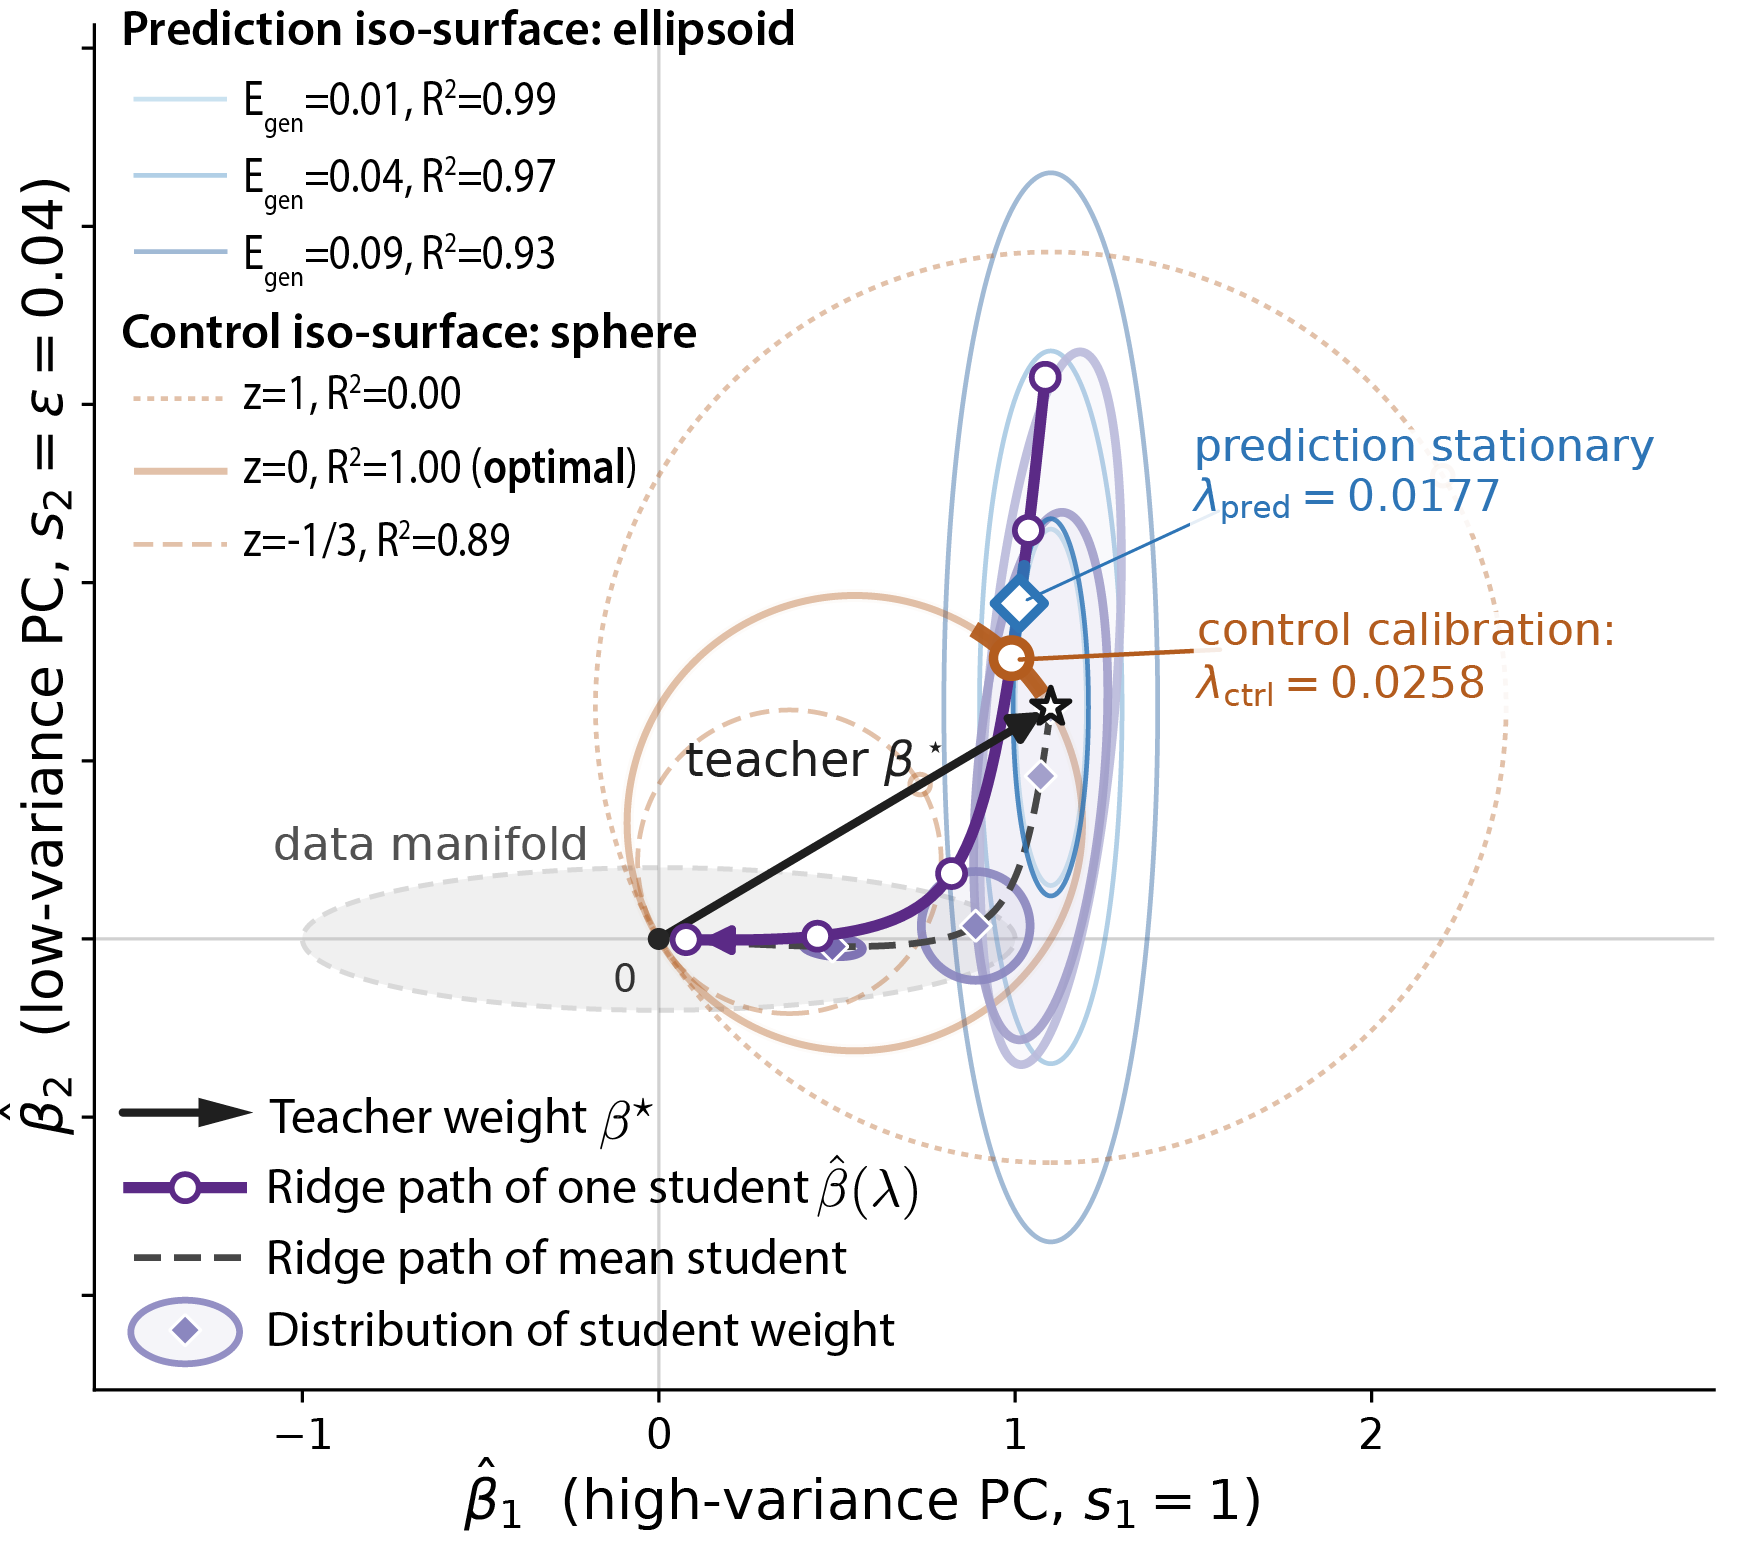
\includegraphics[width=\linewidth]{figures/Figure_iso_err_surf_dissociation-01.png}
    \vspace{-20pt}
    \caption{\textbf{Equal-error sets and the ridge path} in the plane of a high- and a low-variance PC. Prediction levels are ellipsoids around $\bstar$ (blue), control levels are the spheres with diameter joining $0$ and $(1+z)\bstar$ (orange). The fitted weight traverses this plane as a function of $\lambda$ (purple), scattering around the conditional-mean path (dashed black). The prediction-optimal penalty is the tangency of the path with an ellipsoid; perfect control is its crossing with the $z=0$ sphere. Exact two-dimensional construction: App.~\ref{sec:app-ext-geometry}. }
    \label{fig:geometry}
\end{wrapfigure}
The three evaluations therefore have three geometries in the space of student weights (Table~\ref{tab:evaluation-metrics}; Prop.~\ref{prop:mr-iso-geometry}; Fig.~\ref{fig:geometry}).
\textbf{Prediction: ellipsoids.} The equal-$E_{gen}$ sets are ellipsoids centered on $\bstar$ with semi-axis $\sqrt{E_{gen}/s_k}$ along $\uvec_k$, hence elongated along low-variance axes, where large weight errors are cheap.
\textbf{Control: spheres.} The equal-$z_{acc}$ sets are Euclidean spheres whose diameter joins $0$ and $(1+z)\bstar$; the diameter encodes the error directly, and zero-error students live on the sphere through $\bstar$ at $z=0$, not only at $\bstar$ itself.
\textbf{Peer review: hyperplanes.} The equal-$z_{peer}$ sets are hyperplanes normal to the generator $\bprime$, so a peer reviewer is judged only on its component along the peer's path.
A student can sit deep inside a small prediction ellipsoid, lie on a huge control sphere, and still lie on the zero-error hyperplane of a good generator: this is exactly the configuration of Fig.~\ref{fig:phenomena}\textbf{C}, and it can be made arbitrarily extreme by adding weight along a direction with $s_k\to0$ (Exp .~\ref{ex:mr-dissociation}).


The remaining question is therefore not whether the dissociation is possible but when \emph{learning} produces it. We study three ingredients: finite-sample regression on noisy responses, the choice of regularization, and the feature map through which the gradient reaches the pixels. % We take them in turn.

\vspace{-10pt}
\section{Pixel-space ridge: noise, spectrum and regularization}
\label{sec:pixel}

Ridge regression in pixel space, $\bhat=\arg\min_\beta\frac1n\|X\beta-\mathbf y\|^2+\lambda\|\beta\|^2$, yields
\begin{equation}
\bhat=\underbrace{(\hat\Sigma+\lambda I)^{-1}\hat\Sigma\bstar}_{\text{mean: signal shrinkage}}
+\underbrace{\sigma(\hat\Sigma+\lambda I)^{-1}\tfrac1nX^\top\eta}_{\text{noise}},
\qquad \hat\Sigma=X^\top X/n,
\quad
\mathbf y=X\bstar+\sigma \eta
\label{eq:ridge}
\end{equation}
% Since ridge penalizes weight in low-variance directions, one might expect it to remove these control-vulnerable weight components. We ask whether such risk survives the regularization, even with cross-validated penalty.
Since ridge penalizes weight in low-variance directions, one might expect it to remove these control-vulnerable components. We ask whether such control risk survive a cross-validated penalty.

\paragraph{The ridge path through the two landscapes.}
The question has a geometric reading (Fig.~\ref{fig:geometry}). For a given training set, Eq.~\ref{eq:ridge} traces a path $\bhat(\lambda)$ in weight space from the least-squares or minimum-norm solution at $\lambda\to0$ to the origin at $\lambda\to\infty$. Response noise and the random design scatter the fitted weight in a cloud around its mean. Ideally, cross-validation selects the point where the path is tangent to the smallest reachable prediction ellipsoid; whereas minimal control error asks where the path crosses the $z=0$ sphere $D=N$; in general these two points do not coincide. The analysis below makes this geometric picture quantitative.
%\red{the two coincide only if the noise cloud has not pushed the path off the sphere in the directions the ellipsoid does not see. The deterministic equivalents below compute where the center of this cloud sits, how much Euclidean spread it carries, and hence the distance between the two points.}, and the cloud is elongated along the low-variance directions of $\Sigma$, because those are the directions the data constrain least


\paragraph{Toolkit.}
We use deterministic equivalents (DEs) in the proportional limit $d/n\to\gamma$ \citep{dobriban2018high,hastie2022surprises}. They replace functions of the empirical covariance $\hat\Sigma$ by deterministic functions of the population covariance $\Sigma$, e.g. $\hat\Sigma(\hat\Sigma+\lambda I)^{-1}\asymp\Sigma(\Sigma+\kappa I)^{-1}$, where the finite-sample randomness is absorbed into an effective penalty $\kappa(\lambda)\ge\lambda$, the unique positive root of $\kappa-\lambda=\frac{\kappa}{n}\operatorname{Tr}[\Sigma(\Sigma+\kappa I)^{-1}]$, one-to-one in $\lambda$ (App.~\ref{sec:app-de-toolkit}).
Applied to Eq.~\ref{eq:ridge}, the DE says that the signal term concentrates around a \emph{mean fitted weight}, the teacher shrunk mode by mode,
\begin{equation}
\bar\beta_\kappa:=\Sigma(\Sigma+\kappa I)^{-1}\bstar=\sum_k\frac{s_k}{s_k+\kappa}\,b_k\uvec_k ,
\label{eq:pixel-mean-weight}
\end{equation}
% while the noise term has zero mean but carries Euclidean energy,
while the fluctuation around the mean causes the \emph{norm inflation} $V:=\E\|\bhat\|^2-\|\bar\beta\|^2\ge0$, which, as we will show, drives accentuation error. The mean weight $\bar\beta$ and inflation $V$ also organize the feature-space case and the nonlinear diagnostic (Secs.~\ref{sec:feature},~\ref{sec:nonlinear}). Results use the teacher-weighted and unweighted spectral sums
% We use deterministic equivalents (DEs) in the proportional limit $d/n\to\gamma$ \citep{dobriban2018high,hastie2022surprises}. They replace functions of the empirical covariance $\hat\Sigma$ by deterministic functions of the population covariance $\Sigma$, e.g. $\hat\Sigma(\hat\Sigma+\lambda I)^{-1}\asymp\Sigma(\Sigma+\kappa I)^{-1}$, where the finite-sample randomness is absorbed into an effective penalty $\kappa(\lambda)$. $\kappa$ can be found at the unique positive root of $\kappa-\lambda=\frac{\kappa}{n}\operatorname{Tr}[\Sigma(\Sigma+\kappa I)^{-1}]$, with $\kappa\ge\lambda$, and the mapping is one-to-one (App.~\ref{sec:app-de-toolkit}).
% DE allows us to study the average effect of a finite random design without requiring us to manipulate the realized matrix $X$ explicitly.
% Applied to Eq.~\ref{eq:ridge}, the DE says that the signal term concentrates around a \emph{mean fitted weight}, the teacher shrunk mode by mode,
% \begin{equation}
% \bar\beta_\kappa:=\Sigma(\Sigma+\kappa I)^{-1}\bstar=\sum_k\frac{s_k}{s_k+\kappa}\,b_k\uvec_k ,
% \label{eq:pixel-mean-weight}
% \end{equation}
% while the noise term has zero mean, but carries Euclidean energy. We call this energy the \emph{norm inflation}, $V:=\E\|\bhat\|^2-\|\bar\beta\|^2\ge0$. As we will see, it is the part of the fitted weight that can induce severe accentuation error. The same two objects, a mean weight $\bar\beta$ and an inflation $V$, will organize the feature-space case (Sec.~\ref{sec:feature}) and the nonlinear diagnostic (Sec.~\ref{sec:nonlinear}). Results are written with the teacher-weighted and unweighted spectral sums
\begin{equation}\small
B_{p,q}(\kappa)=\sum_k\frac{s_k^p}{(s_k+\kappa)^q}b_k^2,\qquad
\mathrm{df}_{p,q}(\kappa)=\sum_k\frac{s_k^p}{(s_k+\kappa)^q},\qquad \mathrm{df}_2:=\mathrm{df}_{2,2},
\end{equation}
so that, for instance, $\bstar^\top\bar\beta_\kappa=B_{1,1}$ and $\|\bar\beta_\kappa\|^2=B_{2,2}$.
For the ratio $N/D$ we use the leading approximation $\mu_N/\mu_D$ from the DEs of $N$ and $D$; second-order and distributional refinements matter only where the leading calibration error is already small (App.~\ref{sec:app-ratio-corrections}).

\begin{figure}[t]
    \centering
    \vspace{-19pt}
    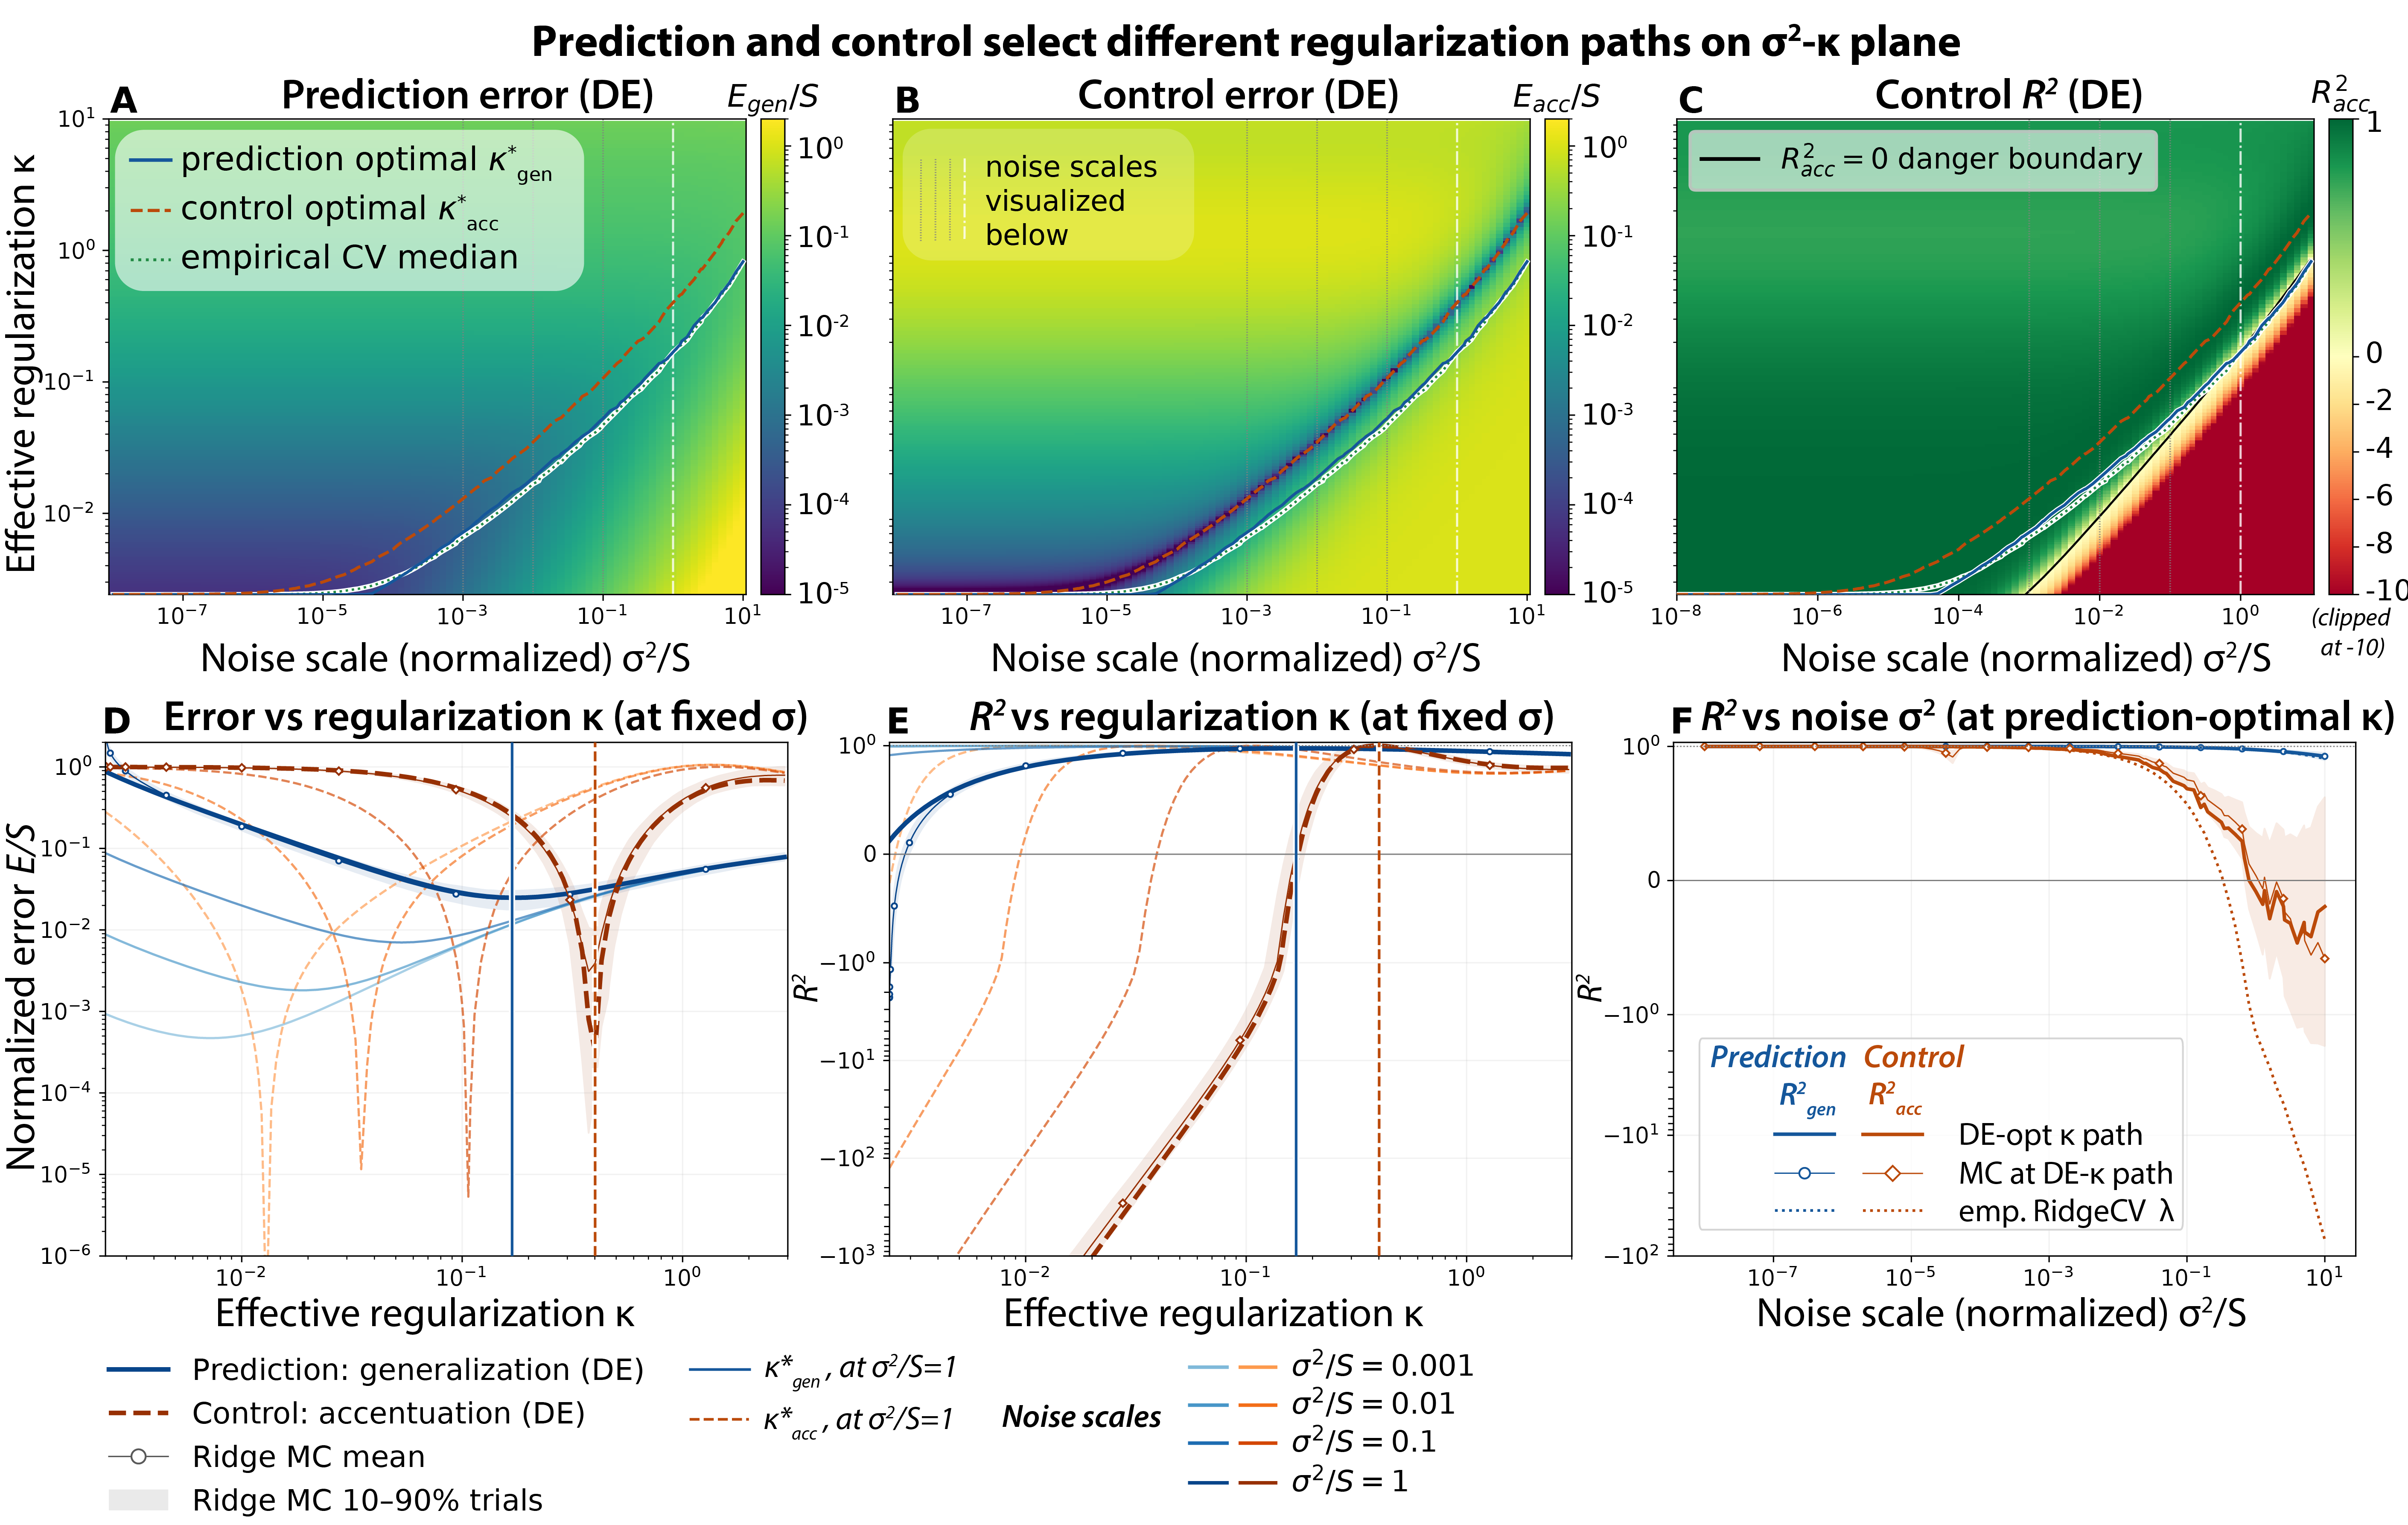
\includegraphics[width=\linewidth]{figures/Figure_PixRidgeGeometry.png}
    \vspace{-15pt}
    \caption{\textbf{Pixel-space ridge separates prediction- and control-optimal regularization on natural images.}
    Disk teacher on van~Hateren images ($d=10^4$, $n=10^3$).
    % \textbf{A--C}~The landscapes of prediction error $E_{gen}$, accentuation error $E_{acc}$, and accentuation $R^2$ over normalized noise scale $\sigma^2/S$ and effective regularization $\kappa$, calculated by DE (Eq.\ref{eq:pixel-de}). The prediction-optimal and median empirical RidgeCV paths track each other but differ from the control-optimal path; the black contour marks $R^2_{acc}=0$.
    % This picture is validated by the numerical MC estimated landscapes in \red{Fig.~\ref{fig:supp-pixel-de-mc}}.
    \textbf{A--C}~DE landscapes (Eq.~\ref{eq:pixel-de}) of $E_{gen}$, $E_{acc}$ and $R^2_{acc}$ over noise $\sigma^2/S$ and effective penalty $\kappa$ (Monte Carlo: Fig.~\ref{fig:supp-pixel-de-mc}). The prediction-optimal and median empirical RidgeCV paths track each other but not the control-optimal path; black contour: $R^2_{acc}=0$.
    \textbf{D,E}~Slices at four noise levels expose displaced prediction and control valleys (or peaks for $R^2$); markers and bands show the mean and 10--90\% range over 100 natural-image trials at the highlighted noise $\sigma^2/S=1$.
    \textbf{F}~Along the prediction-optimal path, $R^2_{gen}$ remains high while $R^2_{acc}$ becomes strongly negative; empirical RidgeCV exhibits the same dissociation. Methods see App.~\ref{sec:app-vanhateren-landscape-methods},~\ref{sec:app-ext-pixel}.}
    \vspace{-15pt}
    \label{fig:pixel}
\end{figure}

\begin{prop}[Pixel ridge: prediction and control]\label{prop:pixel-de}
With $\kappa$, $B$ and $\mathrm{df}$ built from $\Sigma$,
\begin{equation}
\begin{aligned}
E_{gen}&\asymp E_{gen,DE}=\frac{n(\kappa^2B_{1,2}+\sigma^2)}{n-\mathrm{df}_2}-\sigma^2,\qquad
N\asymp \mu_N=\bstar^\top\bar\beta_\kappa=B_{1,1},\\
D&\asymp \mu_D=\|\bar\beta_\kappa\|^2+V_{\rm pix}(\kappa),
\qquad
V_{\rm pix}(\kappa)=\frac{\mathrm{df}_{1,2}(\kappa)}{n}\big(E_{gen,DE}+\sigma^2\big).
\end{aligned}
\label{eq:pixel-de}
\end{equation}
(Proofs and the per-mode decomposition behind these sums: App.~\ref{sec:app-pixel-ridge}.)
\end{prop}
$E_{gen}$ recovers the classical in-distribution generalization error \citep{dobriban2018high,hastie2022surprises}. The two control moments have a plain reading. $N$ is the alignment of the teacher with the mean fitted weight, and the first term of $D$ is that weight's squared norm; both are set by the teacher and the shrinkage alone, and since each factor $s_k/(s_k+\kappa)$ lies in $[0,1]$ they are ordered $\|\bstar\|^2\ge B_{1,1}\ge B_{2,2}$ (Eq.~\ref{eq:app-spectral-inequalities}), so the mean weight by itself \emph{under}-shoots its own path ($D<N$, slope above one). The second term of $D$ is the key issue. $V_{\rm pix}$ summarizes how limited data $n$, response noise $\sigma^2$ and prediction error $E_{gen}$ jointly inflate the student norm, amplified by the spectral susceptibility $\mathrm{df}_{1,2}=\sum_ks_k/(s_k+\kappa)^2$, which counts the number of modes near the regularization threshold $\kappa$.
Inflation enlarges $D$ without changing $N$, so the student can easily \emph{over}-predict: $\mathrm{slope}_{acc}=N/D$ drops below one, and $z=D/N-1$ can grow until $R^2_{acc}=1-z^2$ turns negative.
Note that $V$ is not necessarily bad for control: at the special point $B_{1,1}=B_{2,2}+V_{\rm pix}$ the inflation exactly replenishes the norm lost to shrinkage, so $N=D$ and control is perfect at leading order (the valley in Fig.~\ref{fig:pixel}\textbf{B}).
This is generally not where cross-validation lands, as the next proposition shows.
%that, for a natural-image spectrum, accumulates over thousands of weakly constrained high-frequency modes

\begin{prop}[Prediction-optimal and control-optimal penalties differ]\label{prop:pixel-tuning}
Among admissible values of $\kappa$, let $\kappa_{\rm gen}^{\star}$ be an
interior differentiable minimizer of $E_{\rm gen,DE}$, and let
$\kappa_{\rm acc}^{\star}$ denote a zero of the leading control error,
equivalently satisfying $\mu_D=\mu_N$. Their defining conditions are
\begin{align}\small
E_{\rm gen,DE}+\sigma^2
&=n\kappa\frac{B_{2,3}}{\mathrm{df}_{2,3}},
&&(\kappa=\kappa_{\rm gen}^{\star};\ \text{prediction stationarity}),
\label{eq:gen_optim_reg_cond}\\
E_{\rm gen,DE}+\sigma^2
&=n\kappa\frac{B_{1,2}}{\mathrm{df}_{1,2}},
&&(\kappa=\kappa_{\rm acc}^{\star};\ \text{zero leading control error}).
\label{eq:acc_optim_reg_cond1}
\end{align}
% An interior minimizer of $E_{gen,DE}$ and a zero of the leading control error satisfy, respectively,
% \begin{equation}
% E_{gen,DE}+\sigma^2=n\kappa\frac{B_{2,3}}{\mathrm{df}_{2,3}}
% \quad\text{(prediction)},\qquad
% E_{gen,DE}+\sigma^2=n\kappa\frac{B_{1,2}}{\mathrm{df}_{1,2}}
% \quad\text{(control)},
% \label{eq:acc_optim_reg_cond1}
% \end{equation}
Further, at the prediction optimum $\kappa_{\rm gen}^{\star}$ the control error is
\begin{equation}\small
z^{(0)}_{acc,CV}=\frac{\kappa\,\mathrm{df}_{1,2}}{B_{1,1}}
\left(\frac{B_{2,3}}{\mathrm{df}_{2,3}}-\frac{B_{1,2}}{\mathrm{df}_{1,2}}\right)_{\kappa=\kappa^\star_{gen}} .
\label{eq:pixel-zacc-cv}
\end{equation}
(Proofs: App.~\ref{sec:app-optimal-regularization}.)
\end{prop}
Geometrically, along the ridge path (Fig.~\ref{fig:geometry}), $\kappa_{\rm gen}^{\star}$ lands at the tangency with the prediction ellipsoid and $\kappa_{\rm acc}^{\star}$ at its crossing of the control sphere.
Both conditions equate the noisy prediction risk to $n\kappa$ times a spectral-band average of the teacher's per-mode power $b_k^2$, but the two bands sit at different places (Fig.~\ref{fig:app-tuning-kernels}). The control kernel $s_k/(s_k+\kappa)^2$ is a bump centered at $s_k=\kappa$, symmetric on a log axis; the prediction kernel $s_k^2/(s_k+\kappa)^3$ is the same bump multiplied by the shrinkage factor $s_k/(s_k+\kappa)$, which shifts it up to $s_k\approx2\kappa$ and suppresses its low-variance side.
% \red{Each kernel is a $\kappa$-sensitivity: the control condition asks which modes' shrinkage $s_k/(s_k+\kappa)$ changes as $\kappa$ moves, since that sets the mean weight $\bar\beta_\kappa$ and $N$, whereas prediction stationarity asks which modes' \emph{squared} shrinkage changes, since that sets $E_{gen}$.}
Consequently $z^{(0)}_{acc,CV}$ compares the teacher power around $2\kappa$ with that around $\kappa$.
It vanishes for isotropic data, or for a teacher whose per-mode power $b_k^2$ is constant across modes. % (\todo{Rem.~\ref{rem:app-tuning-remarks}}).
For \textit{an anisotropic spectrum and a structured teacher} the averages differ, and their difference is the control error left at the cross-validated penalty. When $b_k^2$ decreases toward the low-variance tail, as for a teacher aligned with high-variance image modes, $z^{(0)}_{acc,CV}>0$ and the cross-validated student over-predicts ($\mathrm{slope}_{acc}<1$). %For \textit{an anisotropic spectrum and a structured teacher} the two averages differ generally, and their difference is the control error left at the cross-validated penalty. Notably, when $b_k^2$ decreases toward the low-variance tail, as for a teacher aligned with the high variance image modes, $z^{(0)}_{acc,CV}>0$ is positive, and the cross-validated student over-predicts ($\mathrm{slope}_{acc}=1/(1+z)<1$).

% ; and it is negative in the opposite case.
 %teacher-weighted spectral average $B_{,}$, but they average with different powers of $s_k/(s_k+\kappa)$.
% Eq.~\ref{eq:pixel-zacc-cv} is the distance along the path between its tangency with the prediction ellipsoid and its crossing of the control sphere.
%The gap is multiplied by $\kappa\,\mathrm{df}_{1,2}$, i.e. by the number of modes near the regularization edge.

Over the noise--regularization plane for natural images (Fig.~\ref{fig:pixel}\textbf{A--C}), the DE tracks Monte Carlo except at very low noise or regularization (Fig.~\ref{fig:supp-pixel-de-mc}). Prediction- and control-optimal penalties form two distinct valleys, the $E_{acc}$ valley a sharp cusp. At low noise, $\kappa^\star_{\rm gen}$ is also benign to control; as noise grows it approaches and crosses the $R^2_{acc}=0$ cliff, and control fails catastrophically. % tightened
% We visualize the landscape of prediction and control error over the noise-regularization plane ($\sigma^2,\kappa$), for regression on natural images (Fig.~\ref{fig:pixel}A-C).
% Our DE formula generally well tracks the Monte Carlo estimate of the error (Fig.~\ref{fig:supp-pixel-de-mc}), where deviation from leading DE occurs only at very low noise or low regularization cases.
% The prediction-optimal and control-optimal penalties form two distinct valleys, where the $E_{acc}$ valley is a cusp and much sharper than $E_{gen}$.
% At lower noise, prediction-optimal $\kappa^\star_{\rm gen}$ is also benign to control; however, at higher noise, $\kappa^\star_{\rm gen}$ gradually approaches and crosses the cliff of $R^2_{acc}=0$ , and control error fails catastrophically.

% Figure~\ref{fig:pixel} confirms the picture on real natural-image regression. The DE surfaces track Monte Carlo over eight decades of noise; the prediction-optimal and control-calibrated penalties form two distinct ridges; and along the cross-validated path the student remains an excellent predictor while its accentuation $R^2$ becomes negative at moderate noise.

% \red{In Fig.~\ref{fig:geometry}, Eq.~\ref{eq:pixel-zacc-cv} is the distance along the path between its tangency with the prediction ellipsoid and its crossing of the control sphere.}
This answers the question in the title for pixel regression: \emph{control is bad, despite prediction-optimal regularization, when the response is noisy, the spectrum is anisotropic, and many modes sit near $\kappa$}, which is exactly the noisy neuron with natural-image regime.



\paragraph{Peer review: recognition without generation.}
Peer review evaluates $\bhat$ on the path of a peer $\bprime$, so the roles of $N$ and $D$ are played by the true and predicted gains along the peer's path, $N_{peer}={\bstar}^\top\bprime$ and $D_{peer}={\bhat}^\top\bprime$ of Table~\ref{tab:evaluation-metrics}. Take the peer to be a ridge fit at the same $\kappa$ on independent data. Both fits then concentrate around the same mean weight $\bar\beta_\kappa$ while their noise parts are uncorrelated, so the norm inflation drops out of the cross product: $D_{peer}\asymp\|\bar\beta_\kappa\|^2=B_{2,2}$ and $N_{peer}\asymp\bstar^\top\bar\beta_\kappa=B_{1,1}$ (Prop.~\ref{prop:mr-peer}). The peer slope and score are therefore
\begin{equation}
\mathrm{slope}_{peer}=\frac{N_{peer}}{D_{peer}}\asymp\frac{B_{1,1}}{B_{2,2}}\in[1,\infty),
\qquad
R^{2,(0)}_{peer}=1-\Big(1-\frac{B_{2,2}}{B_{1,1}}\Big)^2\in(0,1],
\label{eq:peer-de}
\end{equation}
using $B_{1,1}\ge B_{2,2}$ (Eq.~\ref{eq:app-spectral-inequalities}). Note, on the leading order, the peer slope is never below one, i.e. the \textit{student under-predicts the teacher on its peer's path}, and the peer $R^2$ is non-negative and degrades gracefully with noise through the selected $\kappa$. In contrast, on the self-generated path the norm inflation $V_{\rm pix}$ of Eq.~\ref{eq:pixel-de} adds to $D$ but not to $N$:
%in terms of $z=D/N-1$, $z_{acc}\asymp z_{peer}+V_{\rm pix}/B_{1,1}$ with $z_{peer}=B_{2,2}/B_{1,1}-1\le0$,
so the student over-predicts the teacher ($\mathrm{slope}_{acc}=N/D<1$), and $z_{acc}$ can grow without bound, driving $R^2_{acc}$ negative.
The sign differences in neural data confirm this leading order picture: in \citetPW, peer-review scores between pairs of models have $R^2=0.04,[-0.06,0.10]$, $\mathrm{slope}=1.35,[1.14,1.59]$ (median, [IQR], $n=90$), whereas self-evaluation scores have $R^2=-4.17,[-4.59,-3.51]$, $\mathrm{slope}=0.38,[0.33,0.42]$ ($n=10$; App.~\ref{sec:app-ext-peer}, analysis in App.~\ref{sec:app-methods-peer}). % stats test between the two \todo
Note, in simplistic pixel space peer review, the slope and $R^2$ are symmetric between models ($A\leftarrow B$ or $B\leftarrow A$). In practice the students are fitted to the same recordings through different feature maps; the review score then becomes asymmetric, and the evaluator can recognize its own noise in the generator's path only to the extent that the two maps route noise into the same pixel directions (Sec.~\ref{sec:feature}; App.~\ref{sec:app-peer-shared}).
% Peer review measures only the shared shrinkage bias: at leading order it is never negative, degrades gracefully with noise, and is symmetric between the two fits. Self-evaluation instead carries the estimator's own Euclidean noise energy through Eq.~\ref{eq:pixel-de}, so $z_{acc}$ grows without bound with $\sigma^2/n$ and $R^2_{acc}$ becomes arbitrarily negative. A student can therefore track a peer's path while failing on its own, which is the linear form of Fig.~\ref{fig:phenomena}C.
% The asymmetry between a strong and a weak generator in the data arises when the two differ in their feature maps (Sec.~\ref{sec:feature}); %and measured responses along a barely modulated path add trial noise that no evaluator can explain, which is why even the peer scores of a weak generator's images are poor.

\begin{figure}[tp]
    \centering
    \vspace{-15pt}
    % 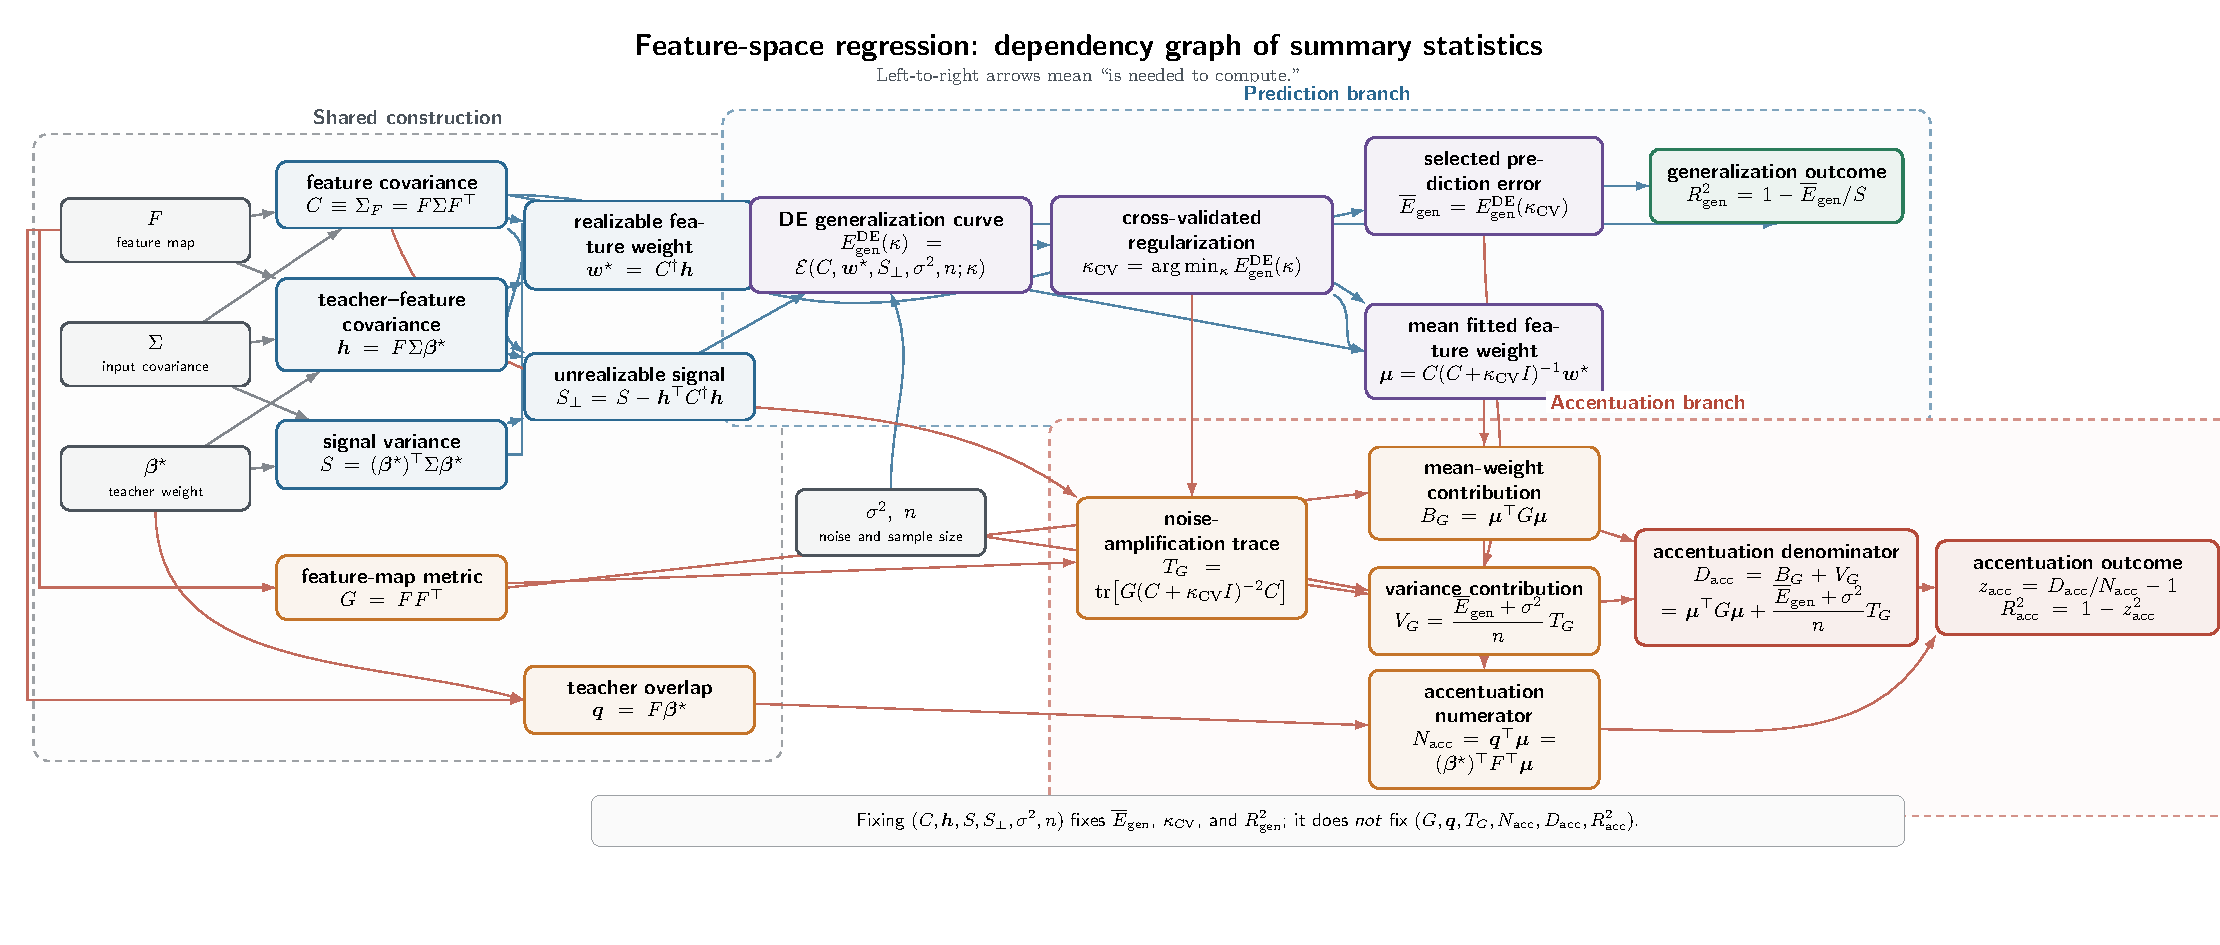
\includegraphics[width=0.55\linewidth,height=0.22\textheight,keepaspectratio]{figures/feature_summary_statistics_flow.pdf}%\hfill
    % 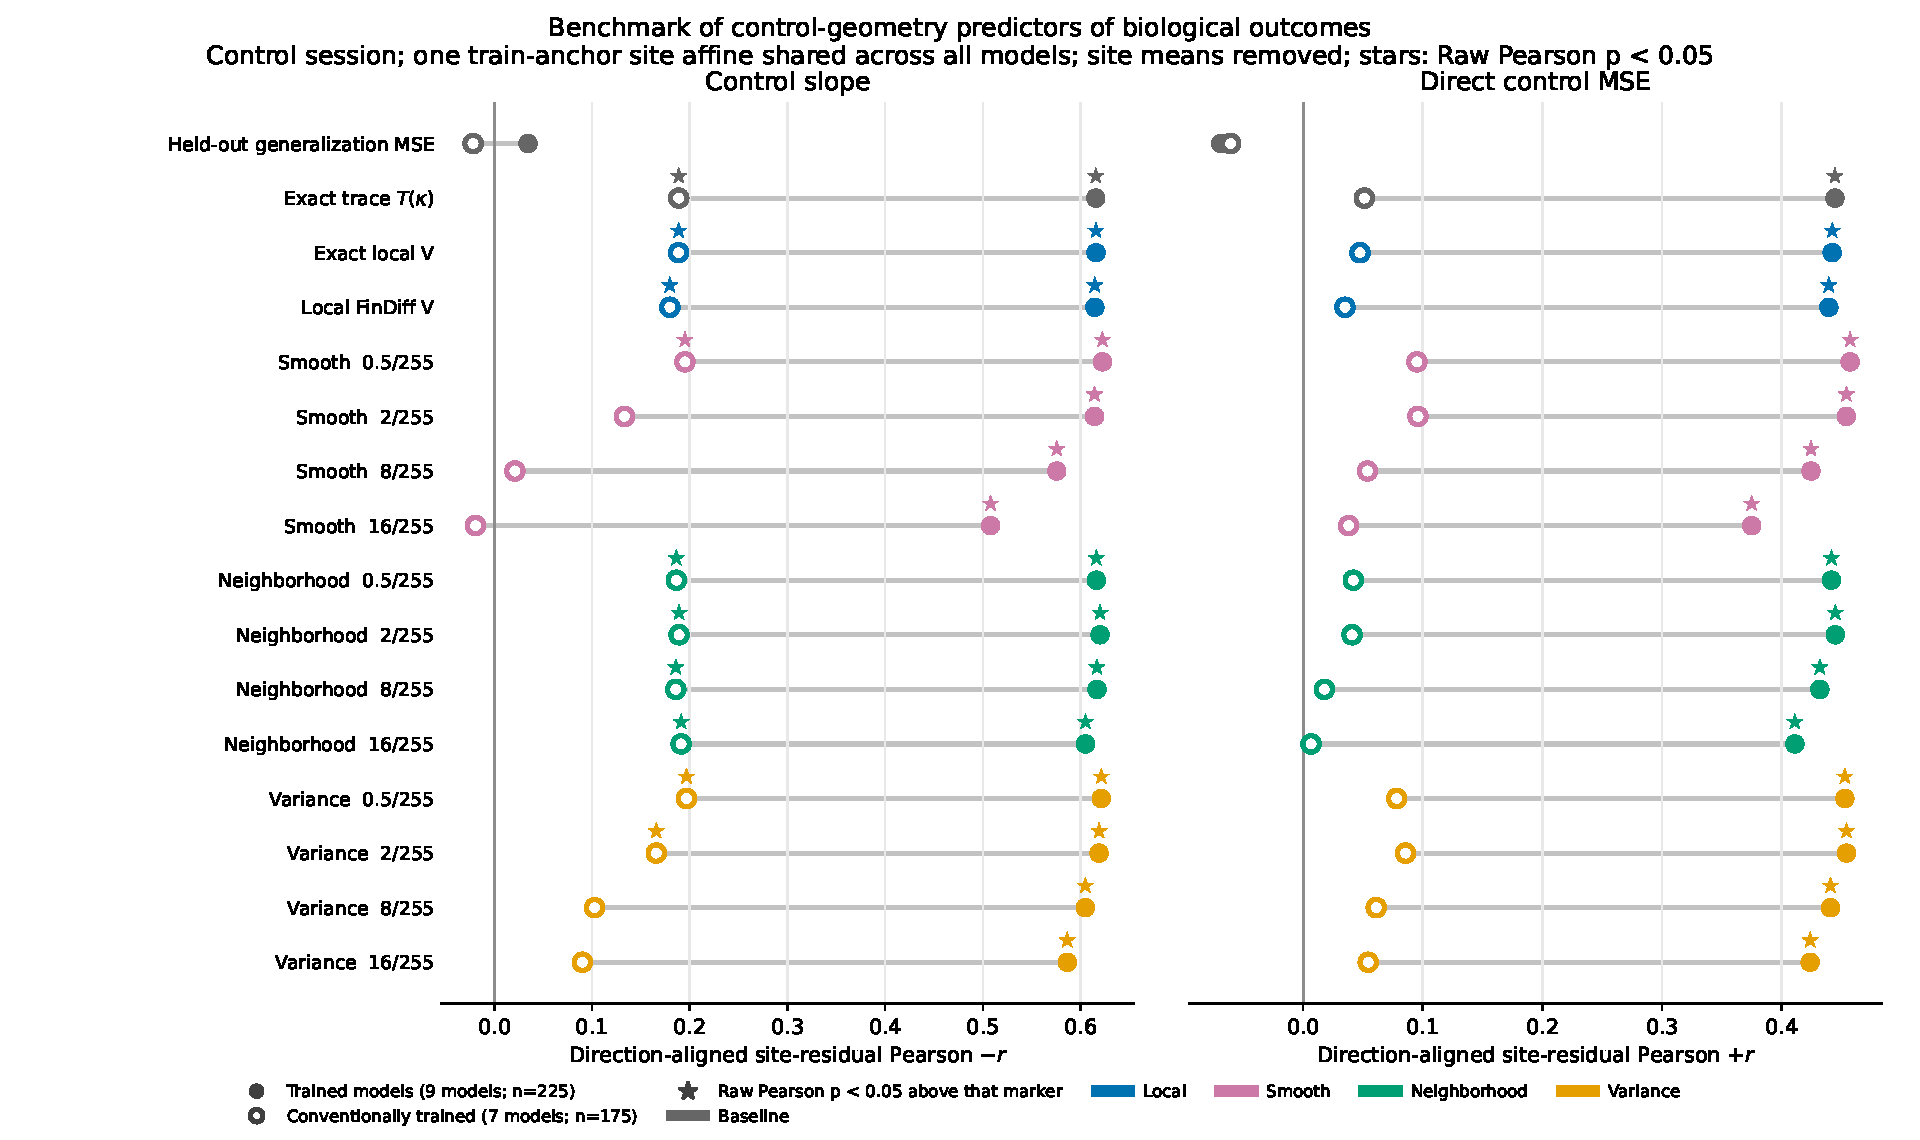
\includegraphics[width=0.44\linewidth,height=0.22\textheight,keepaspectratio]{figures/nonlinear_control_biological_validation.pdf}\\[2pt]
    % 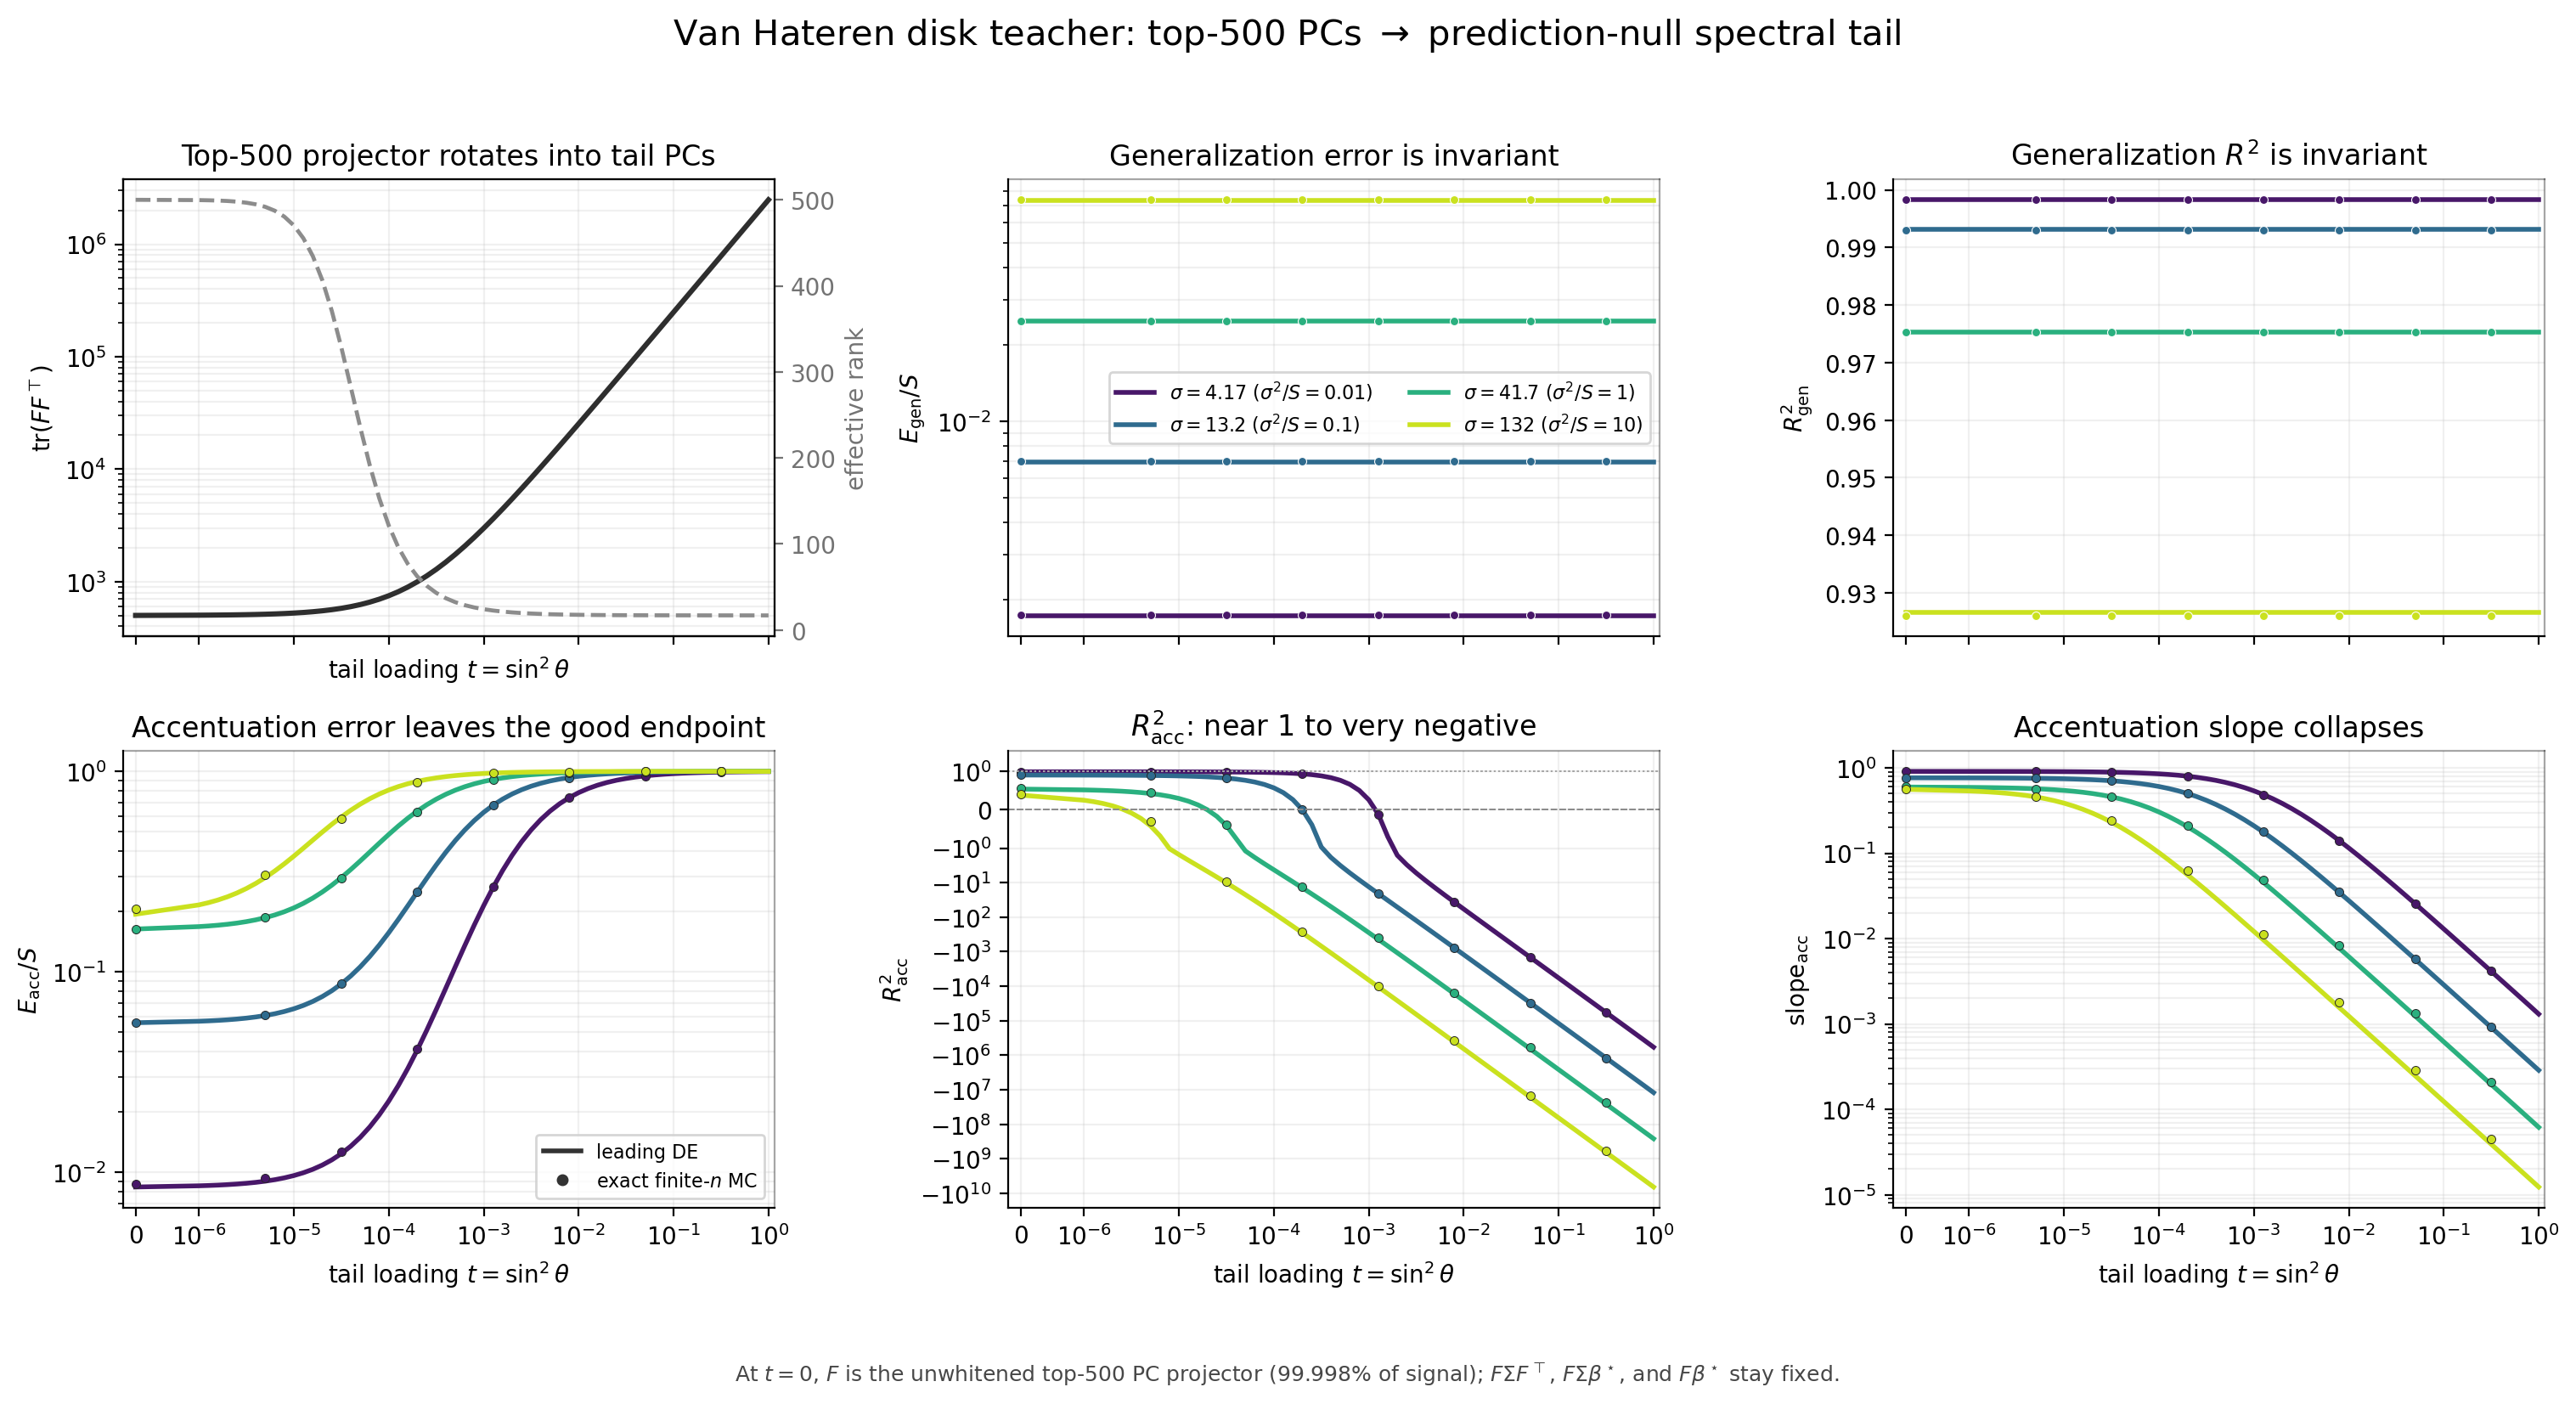
\includegraphics[width=0.45\linewidth,height=0.2\textheight,keepaspectratio]{figures/VanHateren_Top500PC_prediction_null_feature_rotation.png}
    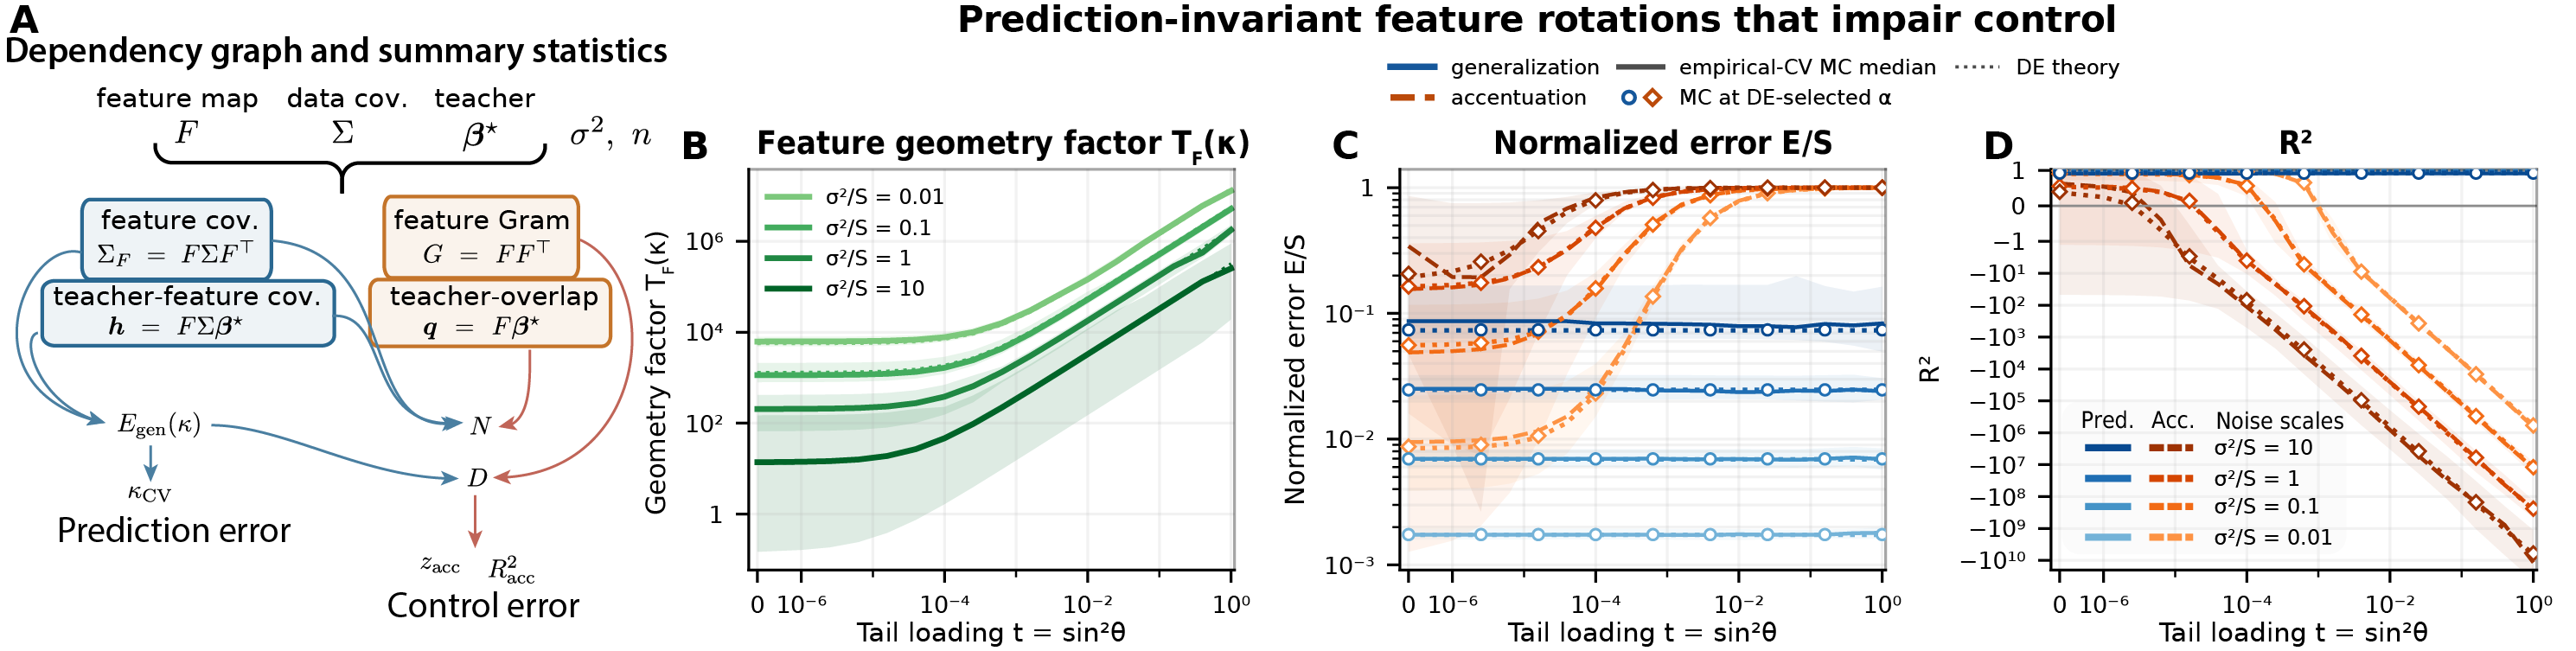
\includegraphics[width=\linewidth]{figures/Figure_linear_feature_gauge.png}
    \vspace{-15pt}
    \caption{\textbf{Feature geometry decides control.}
    \textbf{A}~Dependency graph: $(\Sigma_F,F\Sigma\bstar,S,\sigma^2,n)$ fix generalization and the cross-validated penalty; control additionally needs $\GramDef$ and $F\bstar$ (full graph: Fig.~\ref{fig:summary_stats_dep_graph}).
    \textbf{B-D}~For van Hateren images, rotating the top-500-PC projector feature into the spectral tail: $E_{gen}$ and $R^2_{gen}$ are invariant while $R^2_{acc}$ and the slope collapse; DE (lines) matches Gaussian-design Monte Carlo (markers). Construction: App.~\ref{sec:app-methods-feature}; further rotations: App.~\ref{sec:app-ext-gauge}. }
    %\textbf{C}~Neuronal data: site-demeaned association of each candidate predictor with biological control slope (left) and control error (right) across nine trained (filled) and seven conventionally trained (open) models. Held-out error carries no model-order information; the exact trace, $V_\phi$ and its neighborhood versions do. (Draft: keep 5 rows.)}
    \label{fig:feature}%\label{fig:nonlinear-biological-validation}
\end{figure}
\vspace{-8pt}
\section{Linear feature ridge: effect of gradient geometry} %the map decides what reaches the gradient
\label{sec:feature}

Pixel regression explains why one student fails; it cannot explain why ten equally predictive backbones fail differently. We idealize a backbone as a fixed linear map $F\in\R^{p\times d}$, fit $\hat w$ by ridge on features $F\x$, and accentuate along the pixel gradient $\bhat=F^\top\hat w$. Let $\Sigma_F:=F\Sigma F^\top$ be the feature covariance and $\GramDef$ the Euclidean feature Gram. The best realizable feature weight and its irreducible error are $w^\star=\Sigma_F^\dagger F\Sigma\bstar$ and $S_\perp=S-{w^\star}^\top \Sigma_F w^\star$ (App.~\ref{lem:mr-feature-weights}).

% \begin{prop}[Feature ridge: prediction and control]\label{prop:feature-de}\label{prop:linfeat_acc_ND}\label{prop:linfeat_gen_err}
% With $\kappa$, $B^F$ and $\mathrm{df}^F$ built from $(\Sigma_F,w^\star)$ and aspect ratio $p/n$, the mean fitted pixel weight is the realizable weight shrunk in feature space and back-projected, and the norm inflation carries a map-dependent \emph{gradient-geometry factor} $T_F$:
% \begin{equation}
% \bar\beta_{F,\kappa}:=F^\top(\Sigma_F+\kappa I)^{-1}F\Sigma\bstar,
% \quad
% % V_F(\kappa):=\frac{E_{gen,DE}+\sigma^2}{n}\,T_F(\kappa),
% % \,
% % T_F(\kappa):=\operatorname{Tr}\big[\Gram(\Sigma_F+\kappa I)^{-2}\Sigma_F\big].
% V_F(\kappa):=\frac1n(E_{gen,DE}+\sigma^2)\,\underbrace{\operatorname{Tr}\big[\Gram(\Sigma_F+\kappa I)^{-2}\Sigma_F\big]}_{T_F(\kappa):=},
% \label{eq:feature-mean-variance}
% \end{equation}
% Then
% \begin{equation}
% E_{gen,DE}=\frac{n(\kappa^2B^F_{1,2}+S_\perp+\sigma^2)}{n-\mathrm{df}^F_2}-\sigma^2,
% \qquad
% N_{DE}={\bstar}^\top\bar\beta_{F,\kappa},
% \qquad
% D_{DE}=\|\bar\beta_{F,\kappa}\|^2+V_F(\kappa).
% \label{eq:feature-de}
% \end{equation}
% Setting $F=I$ gives $\bar\beta_{F,\kappa}=\bar\beta_\kappa$ and $T_F=\mathrm{df}_{1,2}$, recovering Prop.~\ref{prop:pixel-de}. (Proofs: App.~\ref{sec:app-feature-regression}.)
% \end{prop}
\begin{prop}[Feature ridge: prediction and control]\label{prop:feature-de}\label{prop:linfeat_acc_ND}\label{prop:linfeat_gen_err}
With $\kappa$, $B^F$ and $\mathrm{df}^F$ built from $(\Sigma_F,w^\star)$ and aspect ratio $p/n$,
\begin{equation}\small
E_{gen,DE}=\frac{n(\kappa^2B^F_{1,2}+S_\perp+\sigma^2)}{n-\mathrm{df}^F_2}-\sigma^2,
\qquad
N_{DE}={\bstar}^\top\bar\beta_{F,\kappa},
\qquad
D_{DE}=\|\bar\beta_{F,\kappa}\|^2+V_F(\kappa).
\label{eq:feature-de}
\end{equation}
where
the mean fitted pixel weight $\bar\beta_{F,\kappa}$ is the realizable weight shrunk in feature space and back-projected, and the norm inflation carries a map-dependent \emph{gradient-geometry factor} $T_F$:
\begin{equation}\small
\bar\beta_{F,\kappa}:=F^\top(\Sigma_F+\kappa I)^{-1}F\Sigma\bstar,
\quad
% V_F(\kappa):=\frac{E_{gen,DE}+\sigma^2}{n}\,T_F(\kappa),
% \,
% T_F(\kappa):=\operatorname{Tr}\big[\Gram(\Sigma_F+\kappa I)^{-2}\Sigma_F\big].
V_F(\kappa):=\frac1n(E_{gen,DE}+\sigma^2)\,\underbrace{\operatorname{Tr}\big[\Gram(\Sigma_F+\kappa I)^{-2}\Sigma_F\big]}_{T_F(\kappa):=},
\label{eq:feature-mean-variance}
\end{equation}
Setting $F=I$ gives $\bar\beta_{F,\kappa}=\bar\beta_\kappa$ and $T_F=\mathrm{df}_{1,2}$, recovering Prop.~\ref{prop:pixel-de}. (Proofs: App.~\ref{sec:app-feature-regression}.)
\end{prop}
The structure is the same as in pixel ridge, so the interpretation carries over: $N$ is the teacher's alignment with the mean weight, $D$ is that weight's norm plus an inflation, and the unrealizable signal $S_\perp$ simply acts as extra response noise. What changes is what determines the two objects. Prediction sees the feature map only through $\Sigma_F$ and $F\Sigma\bstar$: the whole curve $E_{gen,DE}(\kappa)$, hence the cross-validated $\kappa$ and $R^2_{gen}$, is a function of $(\Sigma_F,F\Sigma\bstar,S,\sigma^2,n)$. Control additionally depends on the Gram $\Gram$ and on the teacher overlap $F\bstar$, (Fig.~\ref{fig:feature}\textbf{A}; Cor.~\ref{cor:mr-summary-statistics}). Thus the statistics governing control generically exceed those governing prediction. They coincide only in special cases, for instance white data $\Sigma=I$, where $\Gram=\Sigma_F$ and $F\bstar=F\Sigma\bstar$ (App.~\ref{sec:app-gauge-fragility}).
This extra degree of freedom can be seen clearly through the group that transforms feature map without affecting prediction.
\begin{prop}[Prediction-preserving gauge]\label{prop:gauge}
For $\Sigma\succ0$ and any orthogonal $Q$ with $Q\Sigma^{1/2}\bstar=\Sigma^{1/2}\bstar$, the map $F\mapsto F\Sigma^{1/2}Q\Sigma^{-1/2}$ preserves $\Sigma_F$ and $F\Sigma\bstar$, hence the joint feature--response covariance, $E_{gen,DE}(\kappa)$ and the DE-based prediction-optimal penalty $\kappa^\star_{gen}$, while changing $\Gram$ and $F\bstar$ and therefore control (Prop.~\ref{prop:mr-gauge}; construction in App.~\ref{sec:app-gauge-fragility}).
\end{prop}
Note, the gauge acts nontrivially on control only when the input is anisotropic: in white data, control error is also invariant to this group.
Variation of accentuation error grows with anisotropy. Rotating within it moves feature energy from high-variance to low-variance pixel directions at no cost to prediction (Fig.~\ref{fig:feature}B): along a continuous path, $E_{gen}$, $R^2_{gen}$ and the selected penalty are exactly constant, while $\operatorname{Tr}(FF^\top)$ grows by four orders of magnitude and $R^2_{acc}$ falls from near one to $-10^{8}$.
%\red{Random draws from the \textit{rotation group} span a huge range (Fig.~\ref{fig:supp-null-random}), so a population of equally predictive backbones with widely different control is the generic situation, not a construction.}

% For white data, the accentuation error is also invariant across this gauge group, leading to no dissociation.

\paragraph{What makes a map fragile.}
The response-independent part of $V_F$ is the geometric factor $T_F$, which has the spectral form
\begin{equation}
T_F(\kappa)=\sum_{k:s_k>0}\Big(\frac{s_k}{s_k+\kappa}\Big)^2\frac{\|g_k\|^2}{g_k^\top\Sigma g_k},
\qquad g_k:=F^\top v_k,
\label{eq:TF}
\end{equation}
with $(s_k,v_k)$ the eigenpairs of $\Sigma_F$ (Prop.~\ref{prop:mr-fragility}). It averages, over the feature PCs that survive ridge shrinkage ($s_k^2/(s_k+\kappa)^2\sim1$), the ratio between the Euclidean energy of the backpropagated PC gradient $\|g_k\|^2$ and its energy under the natural-image covariance $g_k^\top\Sigma g_k$. Thus, a map is fragile when its \textit{well-resolved feature directions backpropagate into low-variance, high-spatial-frequency pixel directions}. This is the linear counterpart of the third observation of Sec.~\ref{sec:phenomena}, and it can be computed from the map and the image statistics alone.

% \paragraph{Summary: When is control fragile although prediction is fine?}
% Holding the prediction error fixed, the leading control error (Eqs.~\ref{eq:pixel-de}, \ref{eq:pixel-zacc-cv}, \ref{eq:feature-de}) grows with three separable factors:
% \textbf{(i) noise} $(E_{gen}+\sigma^2)/n$, the estimation-noise level, which is the only factor visible from held-out accuracy;
% \textbf{(ii) spectrum} the mismatch between prediction-optimal and control-optimal penalties, Eq.~\ref{eq:pixel-zacc-cv}, which is zero for white data and grows with anisotropy and with teacher energy in low-variance modes;
% \textbf{(iii) map} $T_F$, the ridge-weighted ratio of Euclidean to natural-covariance gradient energy, a property of the feature map alone.
% Visual neuronal responses are known to be highly noisy \citep{goris2014partitioning,churchland2010stimulus}, meeting (i);
% Natural images make (ii) large for every model; the feature map decides (iii), and equally predictive maps can differ in it without bound.
\paragraph{Summary: When is control fragile although prediction is fine?}
Control fails when the norm inflation $V_F$ overshoots the shrinkage deficit (Eqs.~\ref{eq:pixel-de},~\ref{eq:feature-de}). 
The inflation $V_F=(E_{gen}+\sigma^2)\,T_F(\kappa)/n$ is a product of three factors, 
\textbf{(i) response noise} $E_{gen}+\sigma^2$;
\textbf{(ii) limited data} $1/n$;
\textbf{(iii) gradient geometry} $T_F$, the ratio of Euclidean to covariance-weighted gradient energy, a property of the feature map;
\textbf{(iv) mismatched regularization}: on anisotropic data, the cross-validated penalty is designed for prediction, but not control-optimal and can leave a large control error  (Eq.~\ref{eq:pixel-zacc-cv}).
Held-out accuracy reflects only (i); (iii) and (iv) are invisible to it. Neuronal recordings are noisy and short \citep{goris2014partitioning,churchland2010stimulus}, supplying (i)--(ii); natural images make (iv) large for every model; and the feature map decides (iii), in which equally predictive maps differ without bound.


\begin{figure}[t]
    \centering
    \vspace{-15pt}
    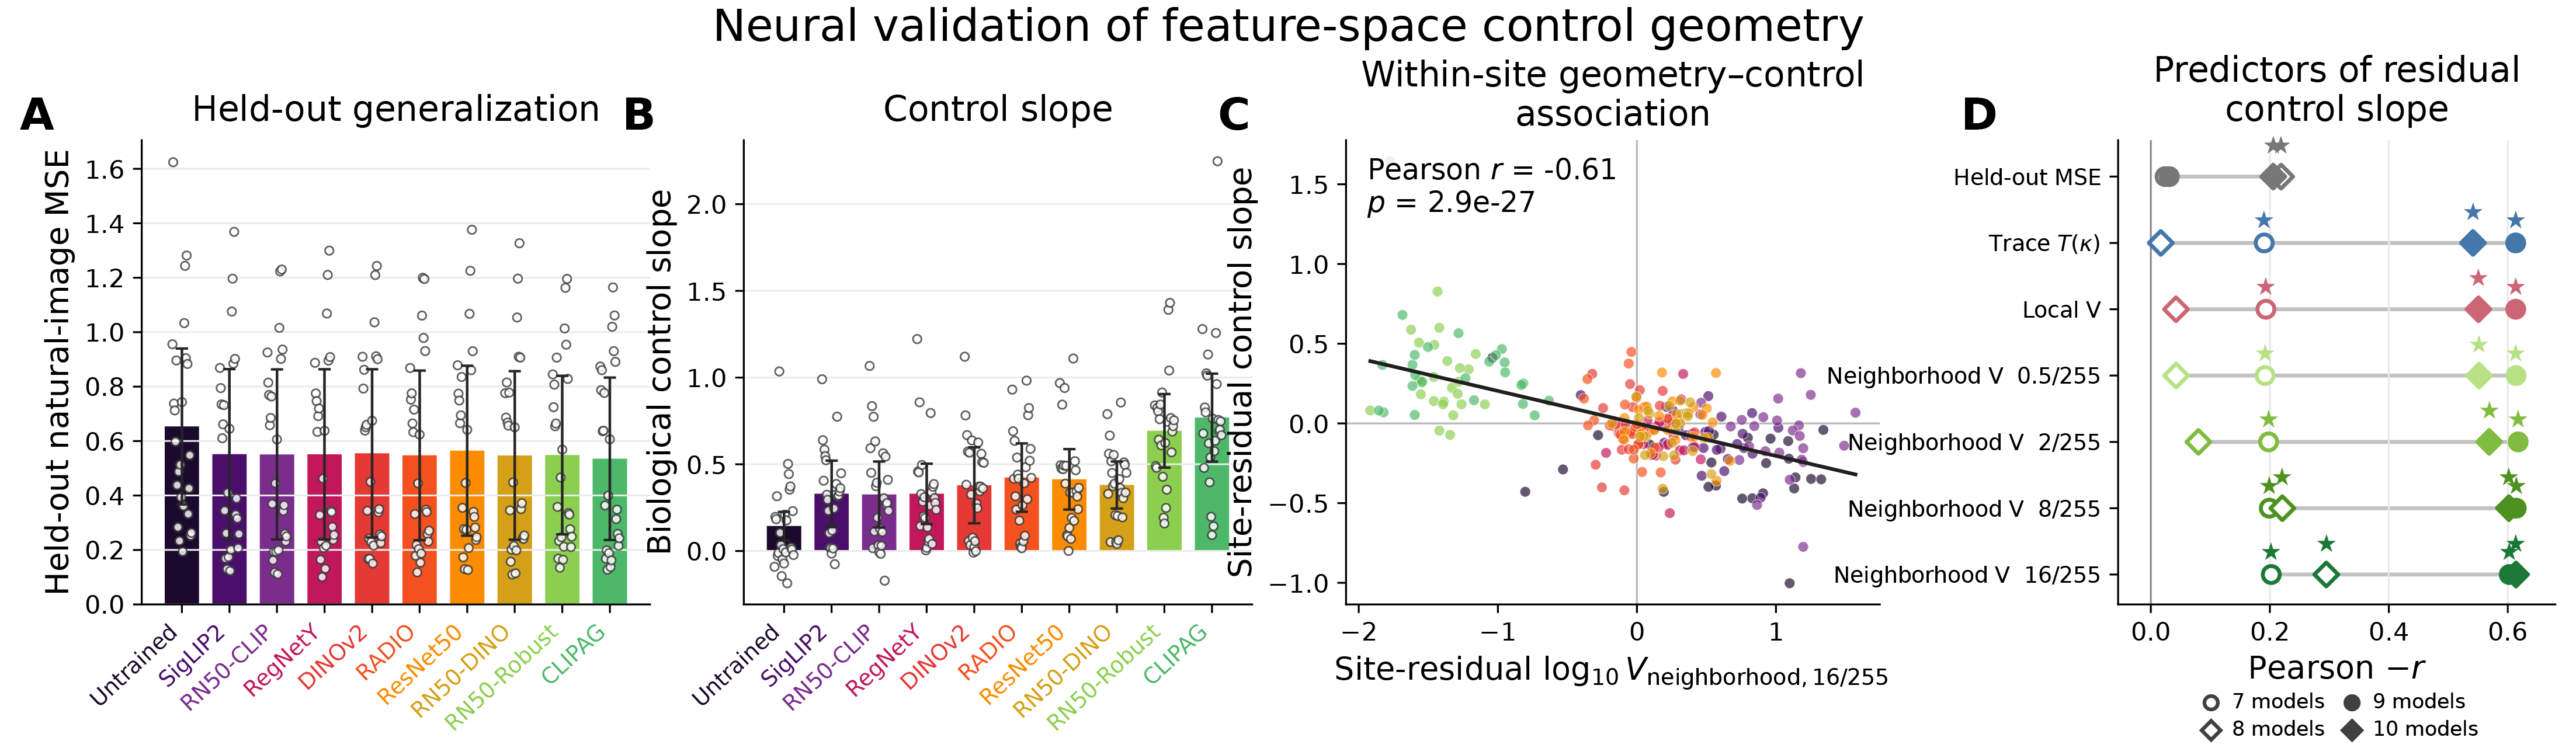
\includegraphics[width=\linewidth]{figures/Figure_nonlinear_neuro_diagnostic.png}
    \vspace{-18pt}
    \caption{\textbf{Gradient-feature geometry in nonlinear model predicts biological control across encoding models.}
% We evaluated ten encoding models at 25 neural recording sites from five subjects. Control-session responses were aligned to the encoding-session scale using a site-specific affine map fitted only on repeated natural-image anchors and shared across models.
% We reproduced the results using published preprocessed data from \citetPW.
% \textbf{A}~MSE on held-out natural-image in the control session, analogous to $E_{\mathrm{val}}\approx E_{\mathrm{gen}}+\sigma^2$.
% \textbf{B}~Control slope between \textit{in vivo} measured and model-predicted neural responses to accentuated stimuli. In \textbf{A,B}, bars show the mean across 25 sites, dots show individual sites, and error bars denote $\pm1$ SE across sites.
% \textbf{C}~Raw $\log_{10}V_\phi$ computed from Jacobian energy averaged over a $16/255$ neighborhood is anticorrelated with control slope after removing each site's ten-model mean (Pearson $r=-0.56$ across 250 site--model pairs).
% \textbf{D}~Pearson correlation ($-r$) between site-centered control slope and seven raw $\log_{10}$ predictors: held-out MSE, the gradient-geometry trace $T_\phi(\kappa)$, exact-local $V_\phi$, and neighborhood $V_\phi$ at four scales.
% Control slope was mean-subtracted within site using all ten models; predictors remained raw. Markers denote 10/9/8/7-model subsets (all / no untrained AlexNet / no robust models (CLIPAG,RN50-robust) / neither), and stars indicate raw two-sided Pearson $p<0.05$. All estimators and scales: App.~\ref{sec:app-ext-nonlinear}.
Published preprocessed data of \citetPW.
\textbf{A}~Held-out natural-image MSE in the control session ($E_{\mathrm{val}}\approx E_{\mathrm{gen}}+\sigma^2$).
\textbf{B}~Slope of observed-over-predicted responses to accentuated stimuli. \textbf{A,B}: mean over 25 sites (bars), sites (dots), $\pm1$ SE.
\textbf{C}~Raw $\log_{10}V_\phi$ ($16/255$ neighborhood) against control slope with each site's ten-model mean removed (Pearson $r=-0.56$, 250 site--model pairs).
\textbf{D}~Pearson $-r$ between site-centered control slope and seven raw $\log_{10}$ predictors (held-out MSE, $T_\phi(\kappa)$, exact-local and neighborhood $V_\phi$ at four scales) for 10/9/8/7-model subsets (all / no untrained AlexNet / no robust models / neither); stars: raw two-sided $p<0.05$. All estimators: App.~\ref{sec:app-ext-nonlinear}.} %without multiple-comparison correction
    \label{fig:nonlinear-biological-validation}
    \vspace{-8pt}
\end{figure}

\vspace{-7pt}
\section{Nonlinear feature ridge: a generalized diagnostic for DNN}
\label{sec:nonlinear}
% Prop.~\ref{prop:feature-de} shows
For linear feature,  $V_F$ is the main culprit of accentuation error. For nonlinear features $\phi$, is there an analogous quantity that preludes control failure?
Viewing a nonlinear feature map $\phi$ as locally linear, we use its Jacobian $J_\phi(x)$ to replace $F$ in Eq.~\ref{eq:TF},
% For a nonlinear feature map $\phi$ with Jacobian $J_\phi(x)$ and natural-image feature covariance eigenpairs $(s_k,v_k)$, replacing $F$ by the local Jacobian gives
\begin{equation}\small
T_\phi(x,\kappa)=\sum_k\frac{s_k}{(s_k+\kappa)^2}\,\|J_\phi(x)^\top v_k\|^2,
\qquad
V_\phi:=\frac{E_{val}}{n}\,\E_x\big[T_\phi(x,\kappa)\big],
\label{eq:Tphi}
\end{equation}
where $(s_k,v_k)$ is the eigenpairs of feature covariance on natural-images, and $J_\phi(x)^\top v_k=\nabla_x[v_k^\top\phi(x)]$ is the pixel gradient of feature PC $k$, obtainable by one backward pass per PC, and $V_\phi$ mirrors the norm inflation $V_F$ of Eq.~\ref{eq:feature-mean-variance} with $E_{val}\approx E_{gen}+\sigma^2$.
Since an accentuation path travels far from the seed, we also evaluate smoothed versions in which the Jacobian is averaged, or the squared gradient is averaged, over a Gaussian neighborhood of the seed at pixel-noise scales from $0.5/255$ to $16/255$ (App.~\ref{sec:app-nonlinear-diagnostic}).
% This is exact for linear $\phi$ and a theory-motivated diagnostic for nonlinear networks. %, where $s_k=g_k^\top\Sigma g_k$ no longer holds.
%For linear $\phi$ this is exact; for a network it is a diagnostic motivated by the theory, because the identity $s_k=g_k^\top\Sigma g_k$ that made $T_F$ a ratio of gradient energies no longer holds.

We computed these quantities for all 250 site--model pairs (App.~\ref{sec:app-methods-nonlinear}), with $\kappa$ set by each model's cross-validated penalty and feature spectrum, average over the ten seed images, and $E_{val}$ the held-out error of the control session. Because sites differ greatly in controllability, {we subtract each site's mean from the control outcome and correlate this residual with the predictors in log10 (Pearson $r$; Fig.~\ref{fig:nonlinear-biological-validation}\textbf{C,D})}. Held-out error carries essentially no ordering information ({$r=0.02$} with control slope, {$-0.04$} with control error, across the nine trained models), whereas exact-local $V_\phi$ reaches {$r=-0.58$ and $+0.40$}; the trace $T_\phi$ alone does {as well ($-0.61$, $+0.43$)}, so the ordering mainly comes from gradient geometry. Among the seven conventionally trained models the slope association is weaker but same-signed ({$r\approx-0.15$ to $-0.17$}): the two adversarially trained models are the strongest controllers and have by far the smallest $T_\phi$. {Neighborhood smoothing ($16/255$) keeps more of the ordering without the robust models ($r=-0.25$ vs.\ $-0.05$ for exact-local $V_\phi$ over eight models).} Thus, the gradient-geometry factor of linear feature maps carries over to deep networks, ranking equally predictive encoding models by \textit{in vivo} control where held-out accuracy cannot. %; the rankings are descriptive, not predictions of absolute control error.% (models repeated within sites)  .

\vspace{-7pt}
\section{Discussion}
\label{sec:discussion}
\vspace{-9pt}
A single mechanism accounts for the three neuronal phenomena: prediction measures weight error in the covariance metric, control measures it along the model's own gradient. In the linear theory the control error at fixed prediction error is governed by the three factors: noise, spectrum, and map, of which only the first is visible from held-out accuracy.
The practical implication is that selecting encoding models or penalties by held-out prediction cannot certify gradient-based control; validation must constrain the gradient, for instance through $T_\phi$, or test generated stimuli directly. The high-frequency artifacts of failed accentuations are not a cosmetic defect but the expected signature of low-variance directions that natural images never constrained.

\paragraph{Limitations.}
The theory assumes Gaussian inputs, a linear teacher, a fixed linear feature map and a linear accentuation path from a centered seed, while some phenomena (e.g. non-trivial Pearson r) requires multiple non-centered seeds.
The details of accentuation procedure (e.g. preconditioning and image prior) could be built in as natural extensions.
The leading DEs predict typical fits and the location of the control optimum but not the fluctuation-dominated error at that optimum (App.~\ref{sec:app-ratio-corrections}).
Our theory did not prove the relation between the diagnostic and control error for nonlinear features; its biological validation is descriptive. %Extending the deterministic equivalents to learned nonlinear features and to curved accentuation trajectories is the natural next step.
